%%\documentclass{../doc/tex/feelstyle}
\documentclass[a4paper]{book}
%\documentclass{article}

\usepackage{a4wide}
\usepackage[utf8]{inputenc}

\usepackage{bm}
\usepackage{textcomp}
%\usepackage{lmodern}
%
%%\usepackage{fullpage}
%\usepackage{venturis2}
\usepackage{newcent}
\usepackage[T1]{fontenc}
\usepackage{longtable}
\usepackage{url}
\usepackage{sectsty}
\sectionfont{\sf}
\subsectionfont{\it}
\usepackage[Sonny]{fncychap}
\usepackage{fancyhdr}
\pagestyle{fancyplain}
\lhead{}
\rhead{}

%\fancyhead[RE,LO]{\leftmark}
%\fancyhead[LE,RO]{\thepage}

\usepackage{fancybox}
%\usepackage{fancyvrb}
%\usepackage{color}
\usepackage{exscale,relsize}
\usepackage{xspace}
\usepackage{multicol}
\usepackage{makeidx}
\usepackage{subfigure}
\usepackage{verbatim}
\usepackage{booktabs}
\usepackage[english]{babel}
\usepackage{tabularx}
\usepackage{times}
\usepackage{subfigure}
\usepackage{graphicx}
\graphicspath{%
  {pdfs/}%
  {pngs/}
}
\usepackage{amsmath,amssymb}

\usepackage{xspace}
\usepackage{tikz}
\usetikzlibrary{arrows,patterns,plotmarks,shapes,snakes,er,3d,automata,backgrounds,topaths,trees,petri,mindmap}

\usepackage[colorinlistoftodos]{todonotes}

%
% les trois parties (front, main et back)
%

\renewcommand\backmatter{%
%  \let\minisommaire\null
  \cleardoublepage
 % \@mainmatterfalse
 % \@frontmatterfalse
  \fancyfoot{}
  \fancyhead[LE]{\bfseries\thepage}
  \fancyhead[RO]{\bfseries\thepage}
  \fancyhead[LO]{\bfseries\rightmark}
  \fancyhead[RE]{\bfseries\leftmark}
 % \renewcommand{\toclevel@chapter}{-1}% pour avoir le bookmark au même niveau
 %                                     % que part
}









%-----------------------------------------------------------------------
% index
\usepackage{index}
%-----------------------------------------------------------------------
%
% espace verticale entre les groupes dans l'index
%
\renewcommand\indexspace{\par \vskip 20pt plus5pt minus3pt\relax}
%-----------------------------------------------------------------------


%-----------------------------------------------------------------------
%
% pour avoir un lien correct dans les bookmark du pdf, sur l'index
%
\let\printindexORIG\printindex
\renewcommand{\printindex}{%
  \cleardoublepage
  \phantomsection% création d'une fausse section
  \addcontentsline{toc}{chapter}{Index}
  \printindexORIG}


\AtBeginDocument{%
  \makeindex%
}

%-----------------------------------------------------------------------


%-----------------------------------------------------------------------
% fancyvrb unixcom environment
\usepackage{styles/fvrb}

%-----------------------------------------------------------------------
% nota environment
\usepackage{styles/nota}
%\newcommand{\ficnota}{attention}
%\newcommand{\ficnota}{}
%\newcommand{\ficnote}{note}
\newcommand{\ficnote}{}
%\newcommand{\ficnotahack}{question}
\newcommand{\ficnotahack}{}

\setlength{\largeurnota}{.8cm}
\newenvironment{nota}{%
  \begin{pictonote}{\ficnota}}{\end{pictonote}}
\newenvironment{note}{%
  \begin{pictonote}{\ficnote}}{\end{pictonote}}
\newenvironment{notahack}{%
  \begin{pictonote}{\ficnotahack}}{\end{pictonote}}


\usepackage{xcolor}
\newtheorem{problem}{Problem}
\newtheorem{remark}{Remark}



\definecolor{lbcolor}{rgb}{0.941,0.984,0.941}
\definecolor{cblue}{rgb}{0.,0.0,0.6}
\definecolor{lblue}{HTML}{045FB4}

\usepackage[colorlinks=true]{hyperref}
\usepackage{filecontents,listings}
\lstset{language=c++,showspaces=false,showstringspaces=false,captionpos=t,literate={>>}{\ensuremath{>>}}1,mathescape}
%\lstset{float}
\lstset{basicstyle=\small\ttfamily}
\lstset{lineskip=-2pt}
\lstset{keywordstyle=\color{red}\bfseries}
%\lstset{keywordstyle=\mdseries\color{red}}
\lstset{emph={inline},emphstyle=\color{red}\bfseries}
\lstset{stringstyle=\ttfamily\color{magenta}}
\lstset{commentstyle=\ttfamily\color{lblue}}
\lstset{backgroundcolor=\color{lbcolor},rulecolor=}
%\lstset{numbers=left}
%\lstset{numbers={none}}
%\lstset{numberstyle=\tiny}
%\lstset{numbersep=1pt}
\lstset{frame=single,framerule=0.5pt}
\lstset{belowskip=\smallskipamount}
\lstset{aboveskip=\smallskipamount}
\lstset{emph={constant,cst,cst_ref,constant_ref,val,integrate,on,grad,gradt,gradv,dot,id,dx,dy,dz,idt,dxt,dyt,dzt,div,divt,idv,dxv,dyv,dzv,dn,dnt,mass,stiffness,trans,trace,jump,jumpt,average,averaget,maxface,project,P,Px,Py,Pz,h,H,Hface,hFace,N,Nx,Ny,Nz,sqrt,sin,cos,min,max,abs,sign,pow,chi,exp,log,form1,form2, FunctionSpace, bases,
prod,element_prod, range, subrange, inner_prod,unite,elements,markedelements,markedfaces,boundaryfaces,faces,internalelements,boundaryelements,edges,boundaryedges,_Q},emphstyle=\color{blue}}
\lstset{includerangemarker=false,rangeprefix=\/\/\#\ ,% curly left brace plus space
  rangesuffix=\ \#}% space plus curly right brace
  \lstset{breaklines=true, breakatwhitespace=true}

\newcommand{\feelchapter}[4]{\chapter{#1 \\ \small{\rm By #3}} \vspace{-1cm}
                              Chapter ref: \textbf{[#4]} \label{chap:#4} \vspace{1cm} \chead[#2]{#3}}
\newcommand{\feelappendix}[2]{\chapter{#1} \chead{#2}}


\newcommand{\acos}{\ensuremath{\mathrm{acos}}\xspace}
\newcommand{\asin}{\ensuremath{\mathrm{asin}}\xspace}
\newcommand{\atan}{\ensuremath{\mathrm{atan}}\xspace}
%\newcommand{\tanh}{\ensuremath{\mathrm{tanh}}\xspace}
\newcommand{\cc}{{\sl\sffamily C}\xspace}
\newcommand{\cpp}{C{\hspace{-.3em}\vspace{-.2em}\tiny++}\xspace}
\newcommand{\polyP}[1]{\ensuremath{\mathbb{P}_{#1}}\xspace}
\newcommand{\feel}{\textsc{Feel++}\xspace}
\newcommand{\Feel}{\textsc{Feel++}\xspace}
\newcommand{\FEEL}{\textsc{Feel++}\xspace}
\newcommand{\cmake}{\texttt{cmake}\xspace}
\newcommand{\ccmake}{\texttt{ccmake}\xspace}


\newcommand{\In}{\operatorname{in}}
\newcommand{\Out}{\operatorname{out}}

\newcommand{\setR}[1]{{\ensuremath{\mathbb{R}^{#1}}}\xspace}
\newcommand{\Om}[1]{{\ensuremath{\Omega^{#1}}}\xspace}
\newcommand{\Omst}{{\ensuremath{\Omega^{\text{st}}}}\xspace}

\newcommand{\aloc}[1]{{\ensuremath{a^{#1}_{\text{loc}}}}\xspace}
\newcommand{\iloc}{{\ensuremath{i_{\text{loc}}}}\xspace}
\newcommand{\jloc}{{\ensuremath{j_{\text{loc}}}}\xspace}
\newcommand{\nldof}{{\ensuremath{N_{\text{localdof}}}}\xspace}
\newcommand{\ngdof}{{\ensuremath{N_{\text{geomdof}}}}\xspace}
\newcommand{\ndof}{{\ensuremath{N_{\text{dof}}}}\xspace}
\newcommand{\nel}{{\ensuremath{N_{\text{el}}}}\xspace}
\newcommand{\PS}[1]{{\ensuremath{\mathbb{P}_N}}\xspace}
\newcommand{\QS}[1]{{\ensuremath{\mathbb{Q}_N}}\xspace}
\newcommand{\GT}[1]{{\ensuremath{\mathcal{T}^{#1}}}\xspace}
\newcommand{\GQ}[1]{{\ensuremath{\mathcal{Q}^{#1}}}\xspace}

%% Macros
\renewcommand{\div}{\operatorname{div}}
\newcommand{\rot}{\operatorname{rot}}

\newcommand{\meter}{\ensuremath{\mathrm{m}}\xspace}

\newcommand{\PP}[1]{{\ensuremath{\mathbb{P}_{#1}}}\xspace}

\newcommand{\pHat}{{\ensuremath{\Hat{p}}}\xspace}
\newcommand{\xHat}{{\ensuremath{\Hat{x}}}\xspace}
\newcommand{\wHat}{{\ensuremath{\Hat{w}}}\xspace}
\newcommand{\THat}{{\ensuremath{\Hat{T}}}\xspace}
\newcommand{\Pk}{\ensuremath{\mathbb{P}_k(K)}\xspace}
\newcommand{\PN}{\ensuremath{\mathbb{P}_N(K)}\xspace}
\newcommand{\Pkmun}{\ensuremath{\mathbb{P}_{k-1}(K)}\xspace}

\newcommand{\bbeta}{\ensuremath{\bm\beta}\xspace}

\InputIfFileExists{version}{}{\def\feelversion{\texttt{x.y.z}}}
\title{Feel Manual\\
A Library for Finite and Spectral Element Methods in 1D, 2D and 3D\\
{\small \feelversion }}
\author{Christophe Prud'homme\thanks{Université de Grenoble,
51, rue des Mathématiques, BP53,38041 Grenoble}}
\date{}

\thispagestyle{empty}
\begin{document}
\thispagestyle{empty}


% \CssFile
% /* css.sty */
% body { width: 75% }
% h1,h2,h3,h4,h5,h6,pre,code,p {font-size: 1em; font-weight: normal; }
% dl,li,dt,dd,h1,h2,h3,h4,h5,h6,pre,form,body,html,p,blockquote,fieldset,input {margin: 0; padding: 0;}
% h2,h3,h4,h5,h6 { color: #B30000; }
% h1 { color: #FFB267; }
% h2 { border-bottom: 1px dotted #FFB267; border-left: 1px dotted #FFB267; }
% h3 { border-bottom: 1px dotted #D95934; }

% div.lstlisting{background: #eee; border: thin solid #000;  }
% div.lstinputlisting{background: #eee; border: thin solid #000; }

% \EndCssFile

%\maketitle
\begin{figure}[!h]
\centering
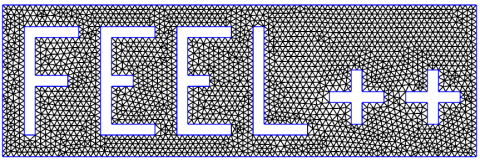
\includegraphics[width=.60\linewidth]{feel_logo.png}
\end{figure}


\begin{center}
  {\Large
    FEEL MANUAL \\
    A LIBRARY FOR \\
    FINITE AND SPECTRAL ELEMENT METHODS IN \\
    1D, 2D AND 3D\\
    \bigskip
    {\small Version \feelversion }}\\[0.6cm]
    Editor\\
  Christophe \textsc{Prud'homme}\\
  \feel Consortium\\
  \texttt{christophe.prudhomme@feelpp.org}\\
  \par\vspace{2cm}

  \begin{flushright}
    \footnotesize
    Date \feeldate\\
    Buildid \feelbuildid
  \end{flushright}
  \par\vspace{5cm}

  % \centerline{\begin{minipage}[l]{0.35\linewidth}
  %   \includegraphics[width=.7\linewidth]{logo-ujf}
  % \end{minipage}
  % \begin{minipage}[r]{0.35\linewidth}
  %   \includegraphics[width=.7\linewidth]{logo-ljk}
  % \end{minipage}}


\end{center}

\vfill \mbox{} \clearpage

\thispagestyle{empty}


\vfill
Permission is granted to copy, distribute and/or modify this document
under the terms of the GNU Free Documentation License, Version 1.2
or any later version published by the Free Software Foundation;
with no Invariant Sections, no Front-Cover Texts, and no Back-Cover Texts.
A copy of the license is included in the section entitled "GNU
Free Documentation License".

\newpage

\tableofcontents

\part{Tutorial}
\label{part:tutorial}

\feelchapter{Crash course}
            {Crash course}
            {Vincent Huber}
            {cha:tutorial-crash-course}

This chapter is designed for impatient people who wants to test \feel as soon as possible.
\section{Requirements}
Before installing \feel, you need to get this \underline{required packages:}\\
\begin{itemize}
\item g++ ($4.4$, $4.5$, $4.6$ or $4.7$) OR Clang ($\geq 3.1$)
\item MPI : openmpi (preferred) or mpich
\item Boost ($\geq$1.39)
\item Petsc ($\geq$2.3.3)
\item Cmake ($\geq$2.6)
\item Gmsh\footnote{Gmsh is a pre/post processing software for scientific
computing available at \url{http://www.geuz.org/gmsh}}
\item Libxml2
\end{itemize}
It is assumed that all this packages are properly installed.

\section{Building \feel from source on *nix}
\feel is distributed as a tarball once in a while. The tarballs are available
at
\begin{center}
  \href{http://code.google.com/p/feelpp/downloads/list}{http://code.google.com/p/feelpp/downloads/list}
\end{center}
Download the latest tarball. Then follow the steps and replace
\texttt{x},\texttt{y},\texttt{z} with the corresponding numbers

\begin{unixcom}
  tar xzf feel-x.y.z.tar.gz
  cd feel-x.y.z
\end{unixcom}
We define then the current directory as the source one, ie:
\begin{unixcom}
  export FeelppSrcDir=`pwd`
\end{unixcom}

\section{Compiling}
Please, notice that 4 Gbytes of RAM is a minimum to make \feel compiling (with \textsc{gcc}), with clang ($\geq 3.1$), the memory footprint is much lower.

In order to compile \feel and a test application, we create a new directory:
\begin{unixcom}
  mkdir build
  cd build
  export buildDir=`pwd`
\end{unixcom}

and then, we are able to compile our first application:
\begin{unixcom}
  cd $buildDir
  cmake $FeelppSrcDir
  make -j4
\end{unixcom}

This procedure will build the entire librarie (with DebWithRelInfo option) and a dummy program to presents the \feel's abilities.

There is a procedure to install as a system librarie \feel.
\begin{unixcom}
  make install
\end{unixcom}
See chapter 2 for more details.

\section{\feel Hello World}
\label{sec:feel-hello-world}

As an introduction to the aim and the way to do with \feel, we provide a sort of
\textit{Hello World} program to evaluate the library.

\subsection{About the math}
\label{sec:about-math}

We want to solve the simplest problem:
\begin{equation}\nonumber
  \begin{aligned}
    - \Delta u &= 1,\\
    u_{|\partial \Omega} &= 0,
  \end{aligned}
\end{equation}
where $\Omega \in \mathbb{R}^n, n\in{1,2,3}$.\\

That problem written in variational form is:
looks for $v\in H^1\left( \Omega \right)$
\begin{equation}\nonumber
  \begin{aligned}
    a\left( u,v \right)&=l\left( v \right)\\
\forall v &\in H^1\left( \Omega \right).
  \end{aligned}
\end{equation}
with:
\begin{equation}\nonumber
  \begin{aligned}
    a\left( u,v \right)&=\int_{\Omega} \nabla u \cdot \nabla v ,\\
    l\left( v \right) &= \int_{\Omega} v .
  \end{aligned}
\end{equation}

The aim of \feel is to provide the simplest way to write the $a$ and $f$ forms.\\

From a discrete point of view, we introduce $V_h\subset H^1\left( \Omega \right)$ such that:
\begin{equation}\nonumber
  \begin{aligned}
V_h = \left\{ v \in C^0\left( \Omega \right), \forall K\in \mathcal{T}_h, \right.v\left|_K \in P_1\left( K \right) \right\},
    \end{aligned}
  \end{equation}
where $\mathcal{T}_h$ is the set of element $K$ forming the mesh of $\Omega$. \\
We now look for $u_h \in V_h$ such that:
\begin{equation}\nonumber
  \begin{aligned}
    \forall v_h\in V_h, a\left( u_h,v_h \right)=l\left( v_h \right).
    \end{aligned}
  \end{equation}

\subsection{About the code}
\label{sec:about-code}

This section is here to declare that we want to use the namespace \feel, to
passe the command line options to the created environnement and add some
informations (basics \feel options, application name).
\lstinputlisting[linerange=marker1-endmarker1]{../../quickstart/laplacian.cpp}
We have to define the mesh, the approximation space and our test and trial
functions.
\lstinputlisting[linerange=marker2-endmarker2]{../../quickstart/laplacian.cpp}
We create now our bilinear and linear forms, we add the homogeneous Dirichlet
conditions and solve the discretized (linear) system.
\lstinputlisting[linerange=marker3-endmarker3]{../../quickstart/laplacian.cpp}
\feel provides the possibility to save the results:
\lstinputlisting[linerange=marker4-endmarker4]{../../quickstart/laplacian.cpp}


\section{First execution \& vizualisation}
\label{sec:first-execution}

To test that part of code, please go to:
\begin{unixcom}
  cd $FeelppSrcDir/quickstart
\end{unixcom}
and execute the code, by:
\begin{unixcom}
  ./feelpp_qs_laplacian
\end{unixcom}
This will produce several files:
\begin{unixcom}
  qs_laplacian-1_0.case
  qs_laplacian-1.sos
  qs_laplacian.timeset
  qs_laplacian.u-1_0.001
  qs_laplacian-1_0.geo001
  qs_laplacian.pid-1_0.001
  square.geo
  square.msh
\end{unixcom}
You can vizualise the results using any Ensight file reader, such as Paraview,
opening \verb=qs_laplacian-1.sos=.
\begin{unixcom}
  paraview qs_laplacian-1.sos
\end{unixcom}
You may have a look to the differents option provided by
\begin{unixcom}
  ./feelpp_qs_laplacian --help
\end{unixcom}


%%% Local Variables:
%%% coding: utf-8
%%% mode: latex
%%% TeX-PDF-mode: t
%%% TeX-parse-self: t
%%% x-symbol-8bits: nil
%%% TeX-auto-regexp-list: TeX-auto-full-regexp-list
%%% TeX-master: "../feel-manual"
%%% ispell-local-dictionary: "american"
%%% End:


\feelchapter{Building Feel++}
            {Building Feel++}
            {Christophe Prud'homme, Baptiste Morin}
            {tutorial-building}

\section{Getting the source via an archive}
\label{sec:getting-source-via-1}

\feel is distributed as a tarball once in a while. The tarballs are available
at
\begin{center}
  \href{http://code.google.com/p/feelpp/}{http://code.google.com/p/feelpp/}
\end{center}
Download the latest tarball.

\begin{unixcom}
  tar -xzf feelpp-0.92.0.tar.gz
  cd feel-0.92.0
\end{unixcom}


\section{Getting the source via Git}
\label{sec:getting-source-via}
In order to download the sources of \feel, you can download it directly from the source depository
thanks to Git. To make it possible, you can download them anonymously or with an account in Github that you have created. As an open-source project, we strongly suggest you to create an account and take part of the project with sharing your ideas, developments or suggests. If you're interested to participate and become a \feel developer, please don't hesitate to see how it works in the appendix ~\ref{feeldevel}. For now, if you want to get the sources without an account, open a command-line and type
\begin{unixcom}
    git clone https://github.com/feelpp/feelpp.git
\end{unixcom}
then you can go to the \feel top directory with
\begin{unixcom}
		cd feel
\end{unixcom}
You should obtain furthers directories such as :
\begin{lstlisting}[language=sh]
applications/   # functional applications
benchmarks/  # applications under test
cmake/   # do not touch, used for compilation
contrib/
doc/   # tutorial and examples
feel/   # Feel++ library
ports/   # used for Mac OS X installation
research/   # research projects using Feel++
testsuite/ # Feel++ unit tests testsuite
CMakeListe.txt   # the file for cmake to build, do not modify
...
\end{lstlisting}

\section{Unix : dependencies}
\label{sec:about-dependencies}

In order to install \feel on Unix systems (other than Mac OS X, in you have a Macintosh, please go to ~\ref{macosx}), you have to install many dependencies
before. Those libraries and programs are necessary for the
compilation and installation of the \feel librairies.
This is the list of all the librairies you must have installed on your
computer, and the \lstinline|*-dev| packages for some of them. \\
\underline{Required packages}:
\begin{itemize}
\item g++ ($4.5$, $4.6$ and $4.7$) or clang++ ($\geqslant 3.1$)
\item MPI : openmpi (preferred) or mpich
\item Boost ($\geq$1.39)
\item Petsc ($\geq$2.3.3)
\item Cmake ($\geq$2.6)
\item Gmsh\footnote{Gmsh is a pre/post processing software for scientific
computing available at \url{http://www.geuz.org/gmsh}}
\item Libxml2
\end{itemize}
\underline{Optional packages}:
\begin{itemize}
\item Superlu
\item Suitesparse(umfpack)
\item Metis: scoth with the metis interface (preferred), metis (non-free)
\item Trilinos ($\geq$8.0.8)
\item Google perftools
\item Paraview\footnote{Paraview is a few parallel scientific data
    visualisation plateform, \url{http://www.paraview.org}}, this is
  not stricly required to run \feel programs but it is somehow
  necessary for visualisation
\item Python ($\geq$ 2.5) for the validation tools
\end{itemize}
Note that all these packages are available under Debian/GNU/Linux and
Ubuntu. They should be available. Once you have installed those dependencies, you can jump to ~\ref{compilingfeel}.

\section{\feel on Debian and Ubuntu}
\label{sec:feel-debian-ubuntu}

\subsection{Debian}

Debian is the platform of choice for \feel, it was developed mainly on it. The commands to install \feel on Debian are
\begin{unixcom}
  sudo apt-get update
  sudo apt-get install feel++-apps libfeel-dev feel++-doc
\end{unixcom}


The interested user is encourage to follow the \feel PTS page
\begin{itemize}
\item \feel \href{http://packages.qa.debian.org/f/feel%2B%2B.html}{Debian Packages Tracking System}
\end{itemize}

At the moment \feel compiles and is available on the following Debian
plateforms:
\begin{itemize}
\item \feel \href{https://buildd.debian.org/status/package.php?p=feel%2b%2b}{Buildd results}
\end{itemize}

\subsection{Ubuntu}

\feel was uploaded in the distribution Ubuntu-Natty (11.04) for the first
time. The commands to install \feel on Ubuntu are
\begin{unixcom}
  sudo apt-get update
  sudo apt-get install feel++-apps libfeel-dev feel++-doc
\end{unixcom}
The interested user might want to follow the Ubuntu Launchpad \feel page in
order to know what is going on with \feel on Ubuntu
\begin{itemize}
\item \feel \href{https://launchpad.net/ubuntu/+source/feel++}{Ubuntu Source
  Page for all Ubuntu versions}
\end{itemize}


\section{\Feel on Mac OS X}
\label{macosx}
\feel is also working on Mac operating systems. The way to make it work is quite different.

\subsection{Compilers}

In order to \feel and \cmake work properly, you have to install differents compilers :
\begin{itemize}
\item Gcc \\
  The first step is to install the latest version of Xcode. If your computer is
  recent, you can install it with your DVD that came with your machine (not the
  OS DVD, but the applications one). You don't have to install the complete
  Xcode (you can uncheck iOS SDK for example, it's not necessary here and
  requiers a lot of memory). Xcode will provide your computer all basic tools to
  compile such as gcc 4.2. It's the first step, you'll see later how to easily
  install gcc 4.5 or later using MacPorts.
\item Fortran \\
  To build the Makefiles, \cmake will need a Fortran compiler. To make it works,
  please go to \href{http://hpc.sourceforge.net/}{SourceForge.net} and download
  \lstinline|gfortran-snwleo-intel-bin.tar.gz| which is the fortran compiler
  only (from now, don't download the complete install with gcc 4.6 because Feel
  needs gcc 4.5 or later). To install it, go to the directory where you have
  downloaded the file and type in a command-line
\begin{unixcom}
		sudo tar -xvf gfortran-snwleo-intel-bin.tar -C /
\end{unixcom}

\end{itemize}

\subsection{MacPorts}

\paragraph{Introduction}
MacPorts is an open-source community projet which aims to design an easy-to-use
system for compiling, installing and upgrading open-source softwares on Mac OS X
operating system. It is distributed under
\href{http://opensource.org/licenses/bsd-license.php}{BSD License} and
facilitate the access to thousands of ports (softwares) without installing or
compiling open-source softwares.  MacPorts provides a single software tree which
includes the latest stable releases of approximately 8050 ports targeting the
current Mac OS X release (10.6 or 10.5). If you want more information, please
visite their \href{http://www.macports.org/}{website}.

\paragraph{Installation}
To install the latest version of MacPorts, please go to
\href{http://www.macports.org/install.php}{Installing MacPorts} page and follow
the instructions. The simplest way is to download the $dmg$ disk image
corresponding to your version of Mac OS X. It is recommended that you install
X11 (X Window System) which is normally used to display X11
applications.%, and also the Xcode Tools (only the developer tools, iOS SDK is not required).

If you have installed with the package installer
(\lstinline|MacPorts-1.x.x.dmg|) that means MacPorts will be installed in
\lstinline|/opt/local|. From now on we will suppose that macports has been
installed in \lstinline|/opt/local| which is the default MacPorts location. Note
that from now on, all tools installed by MacPorts will be installed in
\lstinline!/opt/local/bin! or \lstinline!/opt/local/sbin! for example (that's
here you'll find gcc4.5 or later e.g \lstinline!/opt/local/bin/g++-mp-4.5! once being
installed).%At the end of the installation, you can check if your PATH has been upgraded by the command \lstinline|echo $PATH| which should return a line containing \lstinline|/opt/local/bin:/opt/local/sbin|.

\paragraph{Key commands}
In your command-line, the software MacPorts is called by the command \lstinline|port|.
Here is a list of key commands for using MacPorts, if you want more informations please go to \href{http://guide.macports.org/#using.port}{MacPorts Commands}.
\begin{itemize}
\item \lstinline|sudo port -v selfupdate|
	This action should be used regularly to update the local tree with the global MacPorts ports. The option \lstinline|-v| enables verbose which generates verbose messages.
\item \lstinline|port info flowd|
	This action is used to get information about a port (description, license, maintainer, etc.)
\item \lstinline|sudo port install mypackage|
	This action install the port mypackage
\item \lstinline|sudo port uninstall mypackage|
	This action uninstall the port mypackage
\item \lstinline|port installed|
	This action displays all ports installed and their versions, variants and activation status. You can also use the \lstinline|-v| option to also display the platform and CPU architecture(s) for which the ports were built, and any variants which were explicitly negated.
\item \lstinline|sudo port upgrade mypackage|
	This action updgrades installed ports and their dependencies when a \lstinline|Portfile| in the repository has been updated. To avoid the upgrade of a port's dependencies, use the option \lstinline|-n|.
\end{itemize}

\paragraph{Portfile}
A Portfile is a TCL script which usually contains simple keyword values and TCL
expressions. Each package/port has a corresponding Portfile but it's only a part
of a port description.  \feel provides some mandatory Portfiles for its
compilation which are either not available in MacPorts or are buggy but \feel
also provides some Portfiles which are already available in MacPorts such as
gmsh or petsc. They usually provide either some fixes to ensure \feel works
properly or new version not yet available in MacPorts.  These Portfiles are
installed in \lstinline|ports/macosx/macports|.


\subsection{MacPorts and \Feel}


To be able to install \feel, add the following line in \lstinline|/opt/local/etc/macports/source.conf|
at the top of the file before any other sources :
\begin{lstlisting}[language=sh]
file:///<path to feel top directory>/ports/macosx/macports
\end{lstlisting}

Once it's done, type in a command-line :
\begin{unixcom}
		cd <your path to feel top directory>/ports/macosx/macports
		portindex -f
\end{unixcom}

You should have an output like this :
\begin{flushleft}
\fbox{
   \begin{minipage}{0.81\textwidth}
      	Reading port index in $<$your path to feel top directory$>$/ports/macosx/macports\\
	Adding port science/feel++ \\
	Adding port science/gmsh \\
	Adding port science/petsc \\ \\
	Total number of ports parsed:   3\\
	Ports successfully parsed:      3\\
	Ports failed:                   0\\
	Up-to-date ports skipped:       0
   \end{minipage}
}
\end{flushleft}
Your are now able to type
\begin{unixcom}
		sudo port install feel++
\end{unixcom}
It might take some time (possibly an entire day) to compile all the requirements for \feel
to compile properly. If you have several cores on your MacBook Pro, iMac or MacBook
we suggest that you configure macports to use all or some of them.
To do that uncomment the following line in the file  \lstinline|/opt/local/etc/macports/macports.conf|
\begin{flushleft}
\begin{lstlisting}[language=sh]
buildmakejobs	0 $\#$ all the cores
\end{lstlisting}
\end{flushleft}
At the end of the \lstinline|sudo port install feel++|, you have all
dependencies installed. To build all the Makefile, \cmake is automatically
launched but can have some libraries may not be found but they are not mandatory
for build Feel++, only the features related to the missing libraries will be
missing.

\subsection{PETSc and SLEPc on Snow Leopard and Lion}
We have heard about issues with petsc and slepc with some new MacBook Pro with
Snow Leopard while they are being installed with the command
\begin{unixcom}
  sudo port install feel++
\end{unixcom}
If it's the case, that probably means there is an issue with
atlas. If atlas is already installed, you have to unsinstall it (be careful
with dependencies, they also have to be uninstalled). Once it's done, you should
do
\begin{unixcom}
		cd <path to feel top directory>/ports/macosx/macports
		portindex -f
\end{unixcom}

then type in the exact same order :
\begin{unixcom}
		sudo port uninstall slepc
		sudo port uninstall petsc
		sudo port install -d petsc
		sudo port install slepc
\end{unixcom}
Then add to you shell script environment (e.g. for Bash shells \lstinline|.bashrc| or
\lstinline|.profile| or for CSh shells \lstinline|.tcshrc|)
\begin{unixcom}
  # Sh based shell
  export PETSC_DIR=/opt/local/lib/petsc
  export SLEPC_DIR=/opt/local/lib/petsc

  # CSh based shell
  setenv PETSC_DIR /opt/local/lib/petsc
  setenv SLEPC_DIR /opt/local/lib/petsc
\end{unixcom}
and type once again
\begin{unixcom}
		sudo port install feel++
\end{unixcom}

\noindent In that order, slepc and petsc will be installed before atlas, and feel will be properly installed.

\subsection{Missing ports}
\cmake can build Makefiles even if some packages are missing (latex2html, VTK
...). It's not necessary to install them but you can complete the installation
with MacPorts, \cmake will find them by itself once they have been installed.

\section{Compiling Feel++}
\label{compilingfeel}
Feel build system uses \cmake\index{cmake}\footnote{\url{http://www.cmake.org}}
as its build system. Check that \cmake is using gcc4.5 (or a higher version) 
or clang++ as C++ compiler
(you can use the option \lstinline|CMAKE_CXX_COMPILER=<path>/g++-4.5| where the
\lstinline|path| depends on your OS, it's probably \lstinline|/usr/bin| or
\lstinline|/opt/local/bin| but you can also change it with the command \lstinline|ccmake|
and press \lstinline|t| for advanced options).  
\feel, using \cmake, can be built either in source and out of source and different
build type:
\begin{itemize}
\item minsizerel : minimal size release
\item release release
\item debug : debug
\item none(default)
\end{itemize}

\paragraph{CMake Out Source Build (preferred)}
The best way is to have a directory (\lstinline|FEEL| for example) in which you have : \\
\begin{lstlisting}
	feel/
\end{lstlisting}
where \lstinline|feel| is the top directory where the source have been downloaded. Placed in \lstinline|FEEL|, you can create the build directory (\lstinline|feel.opt| for example) and lauch cmake with :
\begin{unixcom}
  mkdir feel.opt
  cd feel.opt
  cmake <directory where the feel source are>
  # e.g cmake ../feel if feel.opt is at the same
  # directory level as feel
\end{unixcom}
you can customize the build type:
\begin{unixcom}
  # Choose g++ release
  cmake -CMAKE_CXX_COMPILER=/usr/bin/g++-4.5
  # Debug build type (-g...)
  cmake -D CMAKE_BUILD_TYPE=Debug
  # Release build type (-O3...)
  cmake -D CMAKE_BUILD_TYPE=Release
  ...
\end{unixcom}
Once Cmake has made its work, you are now able to compile the library with
\begin{unixcom}
		make
\end{unixcom}
\textbf{Important :} from now, all commands should be type in \lstinline|feel.opt| or its subdirectories.


% \subsection{Compiling Feel with the AutoTools}

% Go in the same folder in wich you have done the checkout and type the following
% commands :

% \subsubsection{From tarball}
% \label{sec:from-tarball}

% The steps are as follows to configure the \feel Development Plateform

% \begin{unixcom}
%   cd feel-x.y.z
%   mkdir opt
%   cd opt

%   ../configure --enable-opt2
% \end{unixcom}

% Then type
% \begin{unixcom}
%   make
% \end{unixcom}

% to compile the library and the tutorial. And finally type
% \begin{unixcom}
%   make check
% \end{unixcom}
% In order to compile the testsuite, the examples and the benchmarks and
% execute some of them to verity that the \feel library is functional.


% \subsubsection{From subversion}
% \label{sec:from-subversion}

% The steps are as follows to configure the \feel Development Plateform

% \begin{unixcom}
%   cd feel
%   make -f Makefile.dist
%   mkdir opt
%   cd opt

%   ../configure --enable-opt2
% \end{unixcom}

% Then, to build  the \feel library, type
% \begin{unixcom}
%   make
% \end{unixcom}

% And finally to check the library, type
% \begin{unixcom}
%   make check
% \end{unixcom}


% \begin{note}
%   The script \lstinline!configure! supports many command line
%   options. In particular if you are interested in writing some code or
%   examples inside the \feel environment you have to enable the so
%   called \emph{maintainer mode} to ensure that the makefiles are
%   properly regenerated when you modify a \lstinline!Makefile.am! or if
%   you modify \lstinline!configure.ac!, to achieve this type
%   \begin{unixcom}
%     configure --enable-maintainer-mode
%   \end{unixcom}
%   To list all configure options, type
%   \begin{unixcom}
%     configure --help
%   \end{unixcom}
% \end{note}


% \subsubsection{Compiling an extra module}
% \label{sec:compile-an-extra}

% If you work with an extra module, \emph{e.g.} \lstinline!validation!, the steps are as follows
% \begin{unixcom}
% cd feel
% make -f Makefile.dist
% cd benchmarks/validation
% make -f Makefile.dist
% cd ../../..
% mkdir opt
% cd opt
% ../feel/configure --enable-opt2 --enable-maintainer-mode
% make
% make check
% \end{unixcom}


\subsection{Compiling the Feel++ manual}
\label{sec:comp-feel-tutor}
The manual (which includes the tutorial) is edited with \LaTeX  so you need to have installed the \LaTeX  distribution on your computer. \LaTeX  is a high-quality typesetting system, it includes features designed for the production of technical and scientific documentation. There are several ways to make it work, for example you can go on \href{http://www.tug.org/mactex/}{MacTeX website} and follow the instructions to install the distribution. If the command \lstinline|make check| in \lstinline|feel.opt/| has been run before, the tutorial
should be already compiled and ready. The steps are as follows to build the Feel tutorial
\begin{unixcom}
  cd feel.opt/doc/manual
  make pdf
\end{unixcom}
%Here is what the directory should look like
%\begin{unixcom}
%  cd opt/doc/tutorial
%  ls
%
%  laplacian     Makefile      myintegrals   mymesh       pngs/
%  tutorial.blg  tutorial.out  tutorial.toc  laplacian.o  myapp
%  myintegrals.o mymesh.o      stokes.assert tutorial.aux pdfs/ styles/
%  stokes        stokes.o      tutorial.bbl  tutorial.log tutorial.pdf
%\end{unixcom}
The directory \lstinline|doc/manual| contains all examples used in the tutorial. You will see how it works in the following parts.

%%% Local Variables:
%%% coding: utf-8
%%% mode: latex
%%% TeX-PDF-mode: t
%%% TeX-parse-self: t
%%% x-symbol-8bits: nil
%%% TeX-auto-regexp-list: TeX-auto-full-regexp-list
%%% TeX-master: "../feel-manual"
%%% ispell-local-dictionary: "american"
%%% End:


\feelchapter{Getting Started with Feel++}
            {Getting Started with Feel++}
            {Christophe Prud'homme, Baptiste Morin, Guillaume Dollé}
            {cha:getting-started}


% first application
% (C) 2013 - Université de Strasbourg
% * Guillaume Dollé <guillaume.dolle@math.unistra.fr>
% * Christophe Prud'homme <christophe.prudhomme@feelpp.org>
% Tutorial documentation - myapp
%


\section{First \feel Application}
\label{sec:myapp}

See section \ref{sec:building} for more information about \feel installation.

\subsection{Minimal example}

Let's begin with our first program using the \feel framework
(source \textcolor{magenta}{"doc/manual/tutorial/myapp.cpp"}).
Before all, you have to include the \feel headers.
%
\vspace{2mm}
\begin{lstlisting}
  #include <feel/feel.hpp>
  using namespace Feel;
\end{lstlisting}
\vspace{2mm}
%
We use the C++ \lstinline!namespace! to avoid \lstinline!Feel::! prefix before
\feel objects.
%
\vspace{2mm}
\lstinputlisting[linerange=marker1-endmarker1]{tutorial/myapp.cpp}
\vspace{2mm}
%
\begin{itemize}
\item
We pass command line options using the
\href{http://www.boost.org/doc/libs/1_53_0/doc/html/program_options.html}
{Boost Program Options}\footnotemark[1] \lstinline!po::! library.
%
\footnotetext[1]{\url{http://www.boost.org/doc/libs/1_53_0/doc/html/program_options.html}}
%
To add a new \feel option, we must create a new
\feel \lstinline!options_description!. You must add the default \feel options
and the new one that we choose here as a double value. Note that the default
value will be assigned if not specified by the user.

\item
Then we initialize the environment variables through the \feel
\lstinline!Environment! class (Check the Constructor prototype on the online documentation).

\item
we instantiate a new application. We specify the directory where to execute the
program. That could be usefull for archiving your results.

\item
Finally, we save the results in a log file using the
\href{http://code.google.com/p/google-glog/}{google-glog library}
\footnotemark[2].
%
\footnotetext{\url{http://code.google.com/p/google-glog/}}
%
As you can see, we save in this example our custom option value and the
current processor number.

\end{itemize}


\subsection{Compilation, execution, logs}

To compile a tutorial, just use the GNU make command.
%
\begin{unixcom}
    make feelpp_doc_<appname>
\end{unixcom}
%
where \textit{appname} is the name of the application you wish to
compile (here, \lstinline!myapp!).
Go to the execution directory as specified in the program,
and execute it. You can change your option value.
%
\begin{unixcom}
    ./feelpp_doc_myapp [--value 6.6]
\end{unixcom}
%
Now if you check the log,
%
\begin{unixcom}
    cat /tmp/<your login>/feelpp_doc_myapp/feelpp_doc_myapp.INFO
\end{unixcom}
%
you should see your value and the processor number used to compute.
You can run your application on several processors using MPI.
%
\begin{unixcom}
    mpirun -np 2 feelpp_doc_myapp
\end{unixcom}
%
Note that there will be one log for each processor in that case.


\subsection{Config files}

A config file can be parsed to the program to profile your options.
The default config paths are,
\begin{enumerate}
    \item current dir
    \item \verb|$HOME/feel/config/|
    \item \verb|$INSTALL_PREFIX/share/feel/config/|
\end{enumerate}
then you have to write inside one of these folders a file called
\lstinline!<app_name>.cfg! or \lstinline!feelpp_<app_name>.cfg!.
For example, our \lstinline!myapp.cfg! would looks like,
%
\vspace{2mm}
\begin{lstlisting}
    value=0.53
\end{lstlisting}
\vspace{2mm}
%
Note that you can specify the config file through the option \lstinline!--config-file=<path>!




\subsection{Initializing PETSc and Trilinos}

\index{PETSc}\index{Trilinos}\index{Libraries!PETSc}\index{Libraries!Trilinos}

PETSc is a suite of data structures and routines for the scalable (parallel)
solution of scientific applications modeled by partial differential
equations. It employs the MPI standard for parallelism.

The Trilinos Project is an effort to develop algorithms and enabling
technologies within an object-oriented software framework for the solution of
large-scale, complex multi-physics engineering and scientific problems.

\feel supports the PETSc and Trilinos framework, the class
\lstinline!Application!\index{Class!Application} takes care of initialize the
associated environments.


% mesh manipulation
% (C) 2013 - Université de Strasbourg
% * Guillaume Dollé <guillaume.dolle@math.unistra.fr>
% * Christophe Prud'homme <christophe.prudhomme@feelpp.org>
% Tutorial documentation - mymesh
%


\section{Mesh Manipulation}
\label{sec:mymesh}

Feel++ provides some tools to manipulate mesh. 
Here is a basic example that shows
you how to generate a mesh for a square geometry
(source \textcolor{magenta}{"doc/manual/tutorial/mymesh.cpp"}).
%
\vspace{2mm}
\lstinputlisting[linerange=marker_main-endmarker_main]{tutorial/mymesh.cpp}
\vspace{2mm}

As always, we initialise the \feel environment (see section \ref{sec:myapp}).
The \lstinline!unitSquare()! will generate a mesh for a square geometry.
\feel provides several functions to automate the GMSH mesh generation
for different topologies.
%
( \lstinline!unitCircle()!,
  \lstinline!unitCube()!,
  \dots ).
%
These functions will create a geometry file
\textit{.geo} and a mesh file \textit{.msh}. We can visualize them in GMSH. 
%
\begin{unixcom}
    gmsh <entity_name>.msh
\end{unixcom}
%
Finally we use the \lstinline!exporter()! function to export the mesh for post processing.
It will create by default a \textbf{Paraview} format file \textit{.sos} and an \textbf{Ensight}
format file \textit{.case}.
%
\begin{unixcom}
    paraview <app_name>.sos
\end{unixcom}
%
For advanced usage, there is the more generic \lstinline!createGMSHMesh()! function which is
useful for creating a mesh from a geometry. For loading a mesh, there is the loadGMSHMesh() function
(see section \ref{howto:spec-meshes} for a load example).
Note that \lstinline!unitSquare()! is just a particular case of \lstinline!createGMSHMesh()!.
\feel provide useful tools to iterate on the mesh or some faces that we will see later.
%
The process of the mesh creation is fully parallelized. You can as explained in section \ref{sec:myapp}
run this example on several processors and visualise subregions with paraview (see figures 
\ref{fig:tuto-mesh-1} and

\begin{figure}[!h]
\centering
\subfigure[Square]
    {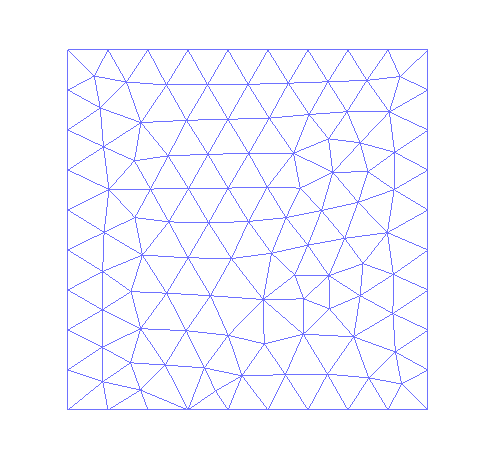
\includegraphics[width=4.5cm]{pngs/mymesh/hypercube_2.png}}
\subfigure[Square and subregions]
    {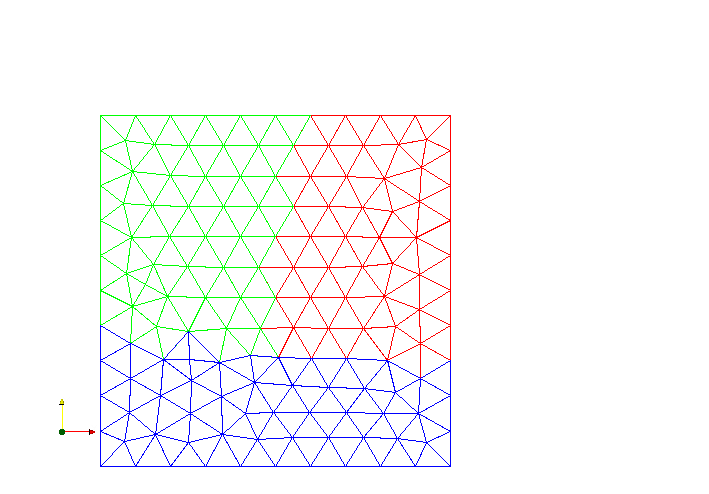
\includegraphics[width=6cm]{pngs/mymesh/mesh3.png}}
\subfigure[Cube ]
    {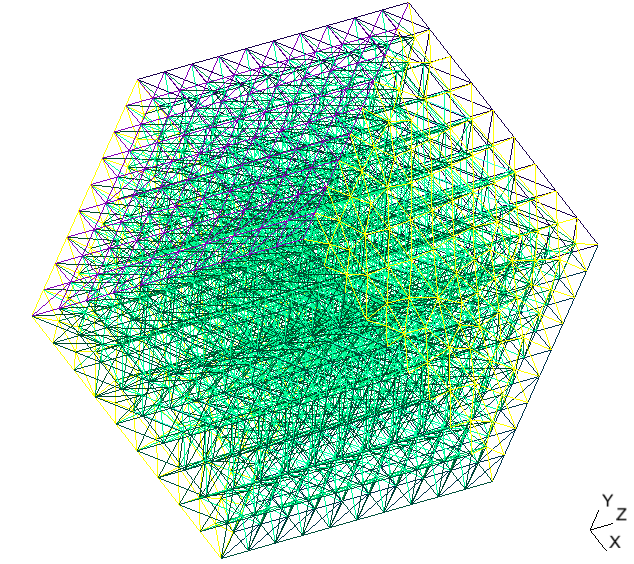
\includegraphics[width=4.5cm]{pngs/mymesh/hypercube_3.png}}
\subfigure[Cube and subregions]
    {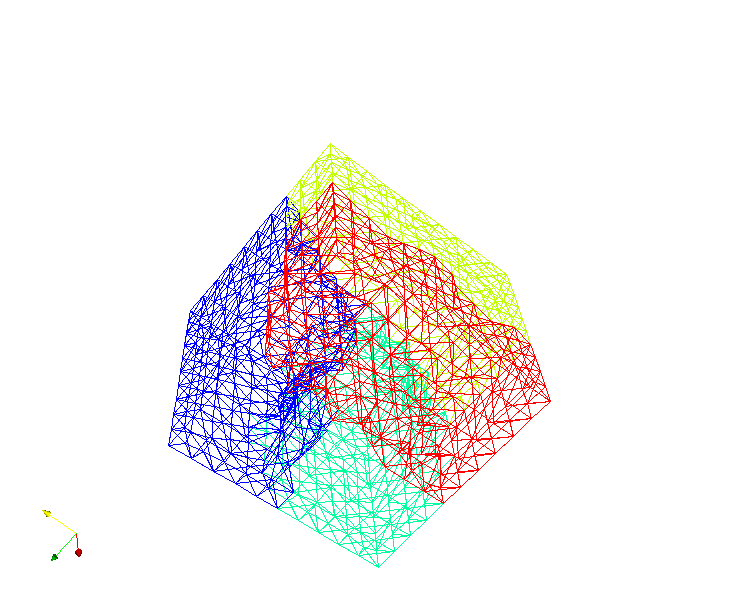
\includegraphics[width=6cm]{pngs/mymesh/mesh_cube.png}}
\end{figure}
\label{fig:tuto_mesh-1}



% integrals computing
% (C) 2013 - Université de Strasbourg
% * Guillaume Dollé <guillaume.dolle@math.unistra.fr>
% * Christophe Prud'homme <christophe.prudhomme@feelpp.org>
% Tutorial documentation - myintegrals
%

\section{Computing Integrals}
\label{sec:myintegrals}

You should be able to create a mesh now. If it is not the case, get back to the
section \ref{sec:mymesh}. This part explains how to integrate on a mesh with \feel
(source \textcolor{magenta}{"doc/manual/tutorial/myintegrals.cpp"}).
Let's consider the domain of the mesh,
\[
    \Omega=[0,1]^d=
    \{
        x\in\mathbb{R}^d\;,\;
        x_i>0\;
        \sum_{i=1}^d x_i \leqslant 1
    \}\in\mathbb{R}^d
\]
Here, we want to integrate the following function,
%
\begin{equation}
    f(x,y,z) = x^2 + y^2 + z^2
\end{equation}
%
on the whole domain $\Omega$ and on part of the boundary $\Omega$. Take a look at the code.
%
\vspace{2mm}
\lstinputlisting[linerange=marker_main-endmarker_main]{tutorial/myintegrals.cpp}
\vspace{2mm}
%
To use the \lstinline!integrate()! function, we have to precise the domain range. You can use,
\begin{itemize}
    \item \lstinline!elements()! to iterate on the whole mesh $\Omega$,
    \item \lstinline!boundaryfaces()! to iterate on the boundary $\partial\Omega$,
    \item \lstinline!markedfaces()! to iterate on a choose face.
\end{itemize}
%
You have to specify the expression we wish to compute. \feel provide a set of functions
to write these expressions \ref{sec:keywords}.
The \lstinline!evaluate()! function computes the integral on the global mesh.
The \lstinline!false! parameter limits the computation on the subregion owned by
the processor.
%
Note that \feel computes automatically the quadrature and consider by default each
non polynomial terms of the expression as a polynomial of degree 2. You can change
it by passing a \lstinline!_quad! parameter to the \lstinline!integrate()! function 
which takes a \lstinline!_Q<int order>! object as value.
(refer to API documentation).





% function spaces
% (C) 2013 - Université de Strasbourg
% * Guillaume Dollé <guillaume.dolle@math.unistra.fr>
% * Christophe Prud'homme <christophe.prudhomme@feelpp.org>
% Tutorial documentation - myfunctionspace
%


\section{Function Spaces}
\label{sec:myfunctionspace}

Now we are able to construct basic \feel applications and compute some integrals 
(If it is not the case, get back to section \ref{sec:mymesh}).
We interest now to solve partial differential equations, so we must define function spaces
to work on. (source \textcolor{magenta}{"doc/manual/tutorial/myfunctionspace.cpp"}).
%
\vspace{2mm}
\lstinputlisting[linerange=marker_main-endmarker_main]{tutorial/myfunctionspace.cpp}
\vspace{2mm}
%
As you can see, we instanciate a new function space object $X_h$ using the \lstinline!Pch<int order>()!
template. These functions are piecewise polynomial of an order precised and the basis functions are
Lagrange polynomials.
Let $g$ be a function such as,
%
\[
    g= \sin(\frac{\pi x}{2}).\cos(\frac{\pi x}{2}).\cos(\frac{\pi z}{2}) \;.
\]
%
For $u,w\in X_h$, we build the Lagrange interpolant. We use for this the
\lstinline!vf::project()! function  which returns the projection on the mesh node for
an expression given as parameter. Then we compute the L2 norm,
%
\[
    \| g \|_2 =
    \sqrt{\left( \int_\Omega g^2 \right)} \;,
\]
%
and the error $\| g - g_{X_h}\|_2$
using the \lstinline!normL2()! function.
Finally, we export our elements $u,w\in X_h$ to visualize them with paraview.
To do so, we have to add them to the exporter.



% solve laplacian dirichlet homogene
% (C) 2013 - Université de Strasbourg
% * Guillaume Dollé <guillaume.dolle@math.unistra.fr>
% * Christophe Prud'homme <christophe.prudhomme@feelpp.org>
% Tutorial documentation - mymesh
%


\section{Laplacian Problem}
\label{sec:tuto-mylaplacian}

This part explains how to solve the Laplacian equation 
for homogeneous dirichlet conditions,
%
\begin{equation}
\left\{
\begin{array}{rcll}
    -\Delta u & = & f & \text{on}\;\Omega \;, \\
            u & = & 0 & \text{on}\;\partial\Omega \;,\\
\end{array}
\right.
\label{eq:tuto-mylaplacian-prob}
\end{equation}
%
where $u\in\Omega$ is the unknown "trial" function and $\Omega$ the domain.
%
We multiply each part of the first equation by a "test" function $v\in H_0^1(\Omega)$ 
and we integrate the resulting equation on the domain $\Omega$,
%
\begin{equation}
-\int_\Omega \Delta u v = \int_\Omega f v \;.
\end{equation}
%
We can integrate by parts this equation (Green Theorem) to obtain \underline{the variationnal
formulation},
%
\begin{equation}
\int_\Omega \nabla u \nabla v
-\underbrace{ \int_{\partial\Omega} \frac{\partial u}{\partial n} v }_{= 0}
=\int_\Omega f v \;,
\end{equation}
%
where $n$ denotes a unit outward normal vector to the boundary. We can rewrite the problem
(\ref{eq:tuto-mylaplacian-prob}) as find $u\in H_0^1(\Omega)$ such that for all
$v\in H_0^1(\Omega)$,
%
\begin{equation}
a(u,v)=l(v) \;,
\end{equation}
where $a$ is a bilinear form, continuous, coercive and $l$ a linear form.
Let's take a look at the \feel code
(source \textcolor{magenta}{"doc/manual/tutorial/mylaplacian.cpp"}).
We consider for this example $f=1$ constant.
%
\vspace{2mm}
\lstinputlisting[linerange=marker_main-endmarker_main]{tutorial/mylaplacian.cpp}
\vspace{2mm}
%
As you can see, the program looks very close to the mathematical formulation.
We use the \lstinline!form2()! function to define the bilinear form and \lstinline!form1()!
for the linear one. The gradient for the trial functions is declared with the \lstinline!gradt()!
expression where as \lstinline!grad()! is used for the test functions
(see all keywords \ref{sec:keywords}).
Note that we need to transpose the second vector to perform the scalar product.
To introduce the homogeneous dirichlet conditions on the boundary, we use the function
\lstinline!on()!. Once the variationnal formulation and the boundary conditions are set, we call
the solver with \lstinline!solve()!.








% solve stokes poiseuille flow
constant-null-space=1
ksp-monitor=1


[gmsh]
gmsh.hsize=0.5

[gmsh.domain]
shape=hypercube
xmin=0
xmax=4
ymin=0
ymax=1

[functions]
alpha=y*(1-y)
beta=0
gamma=(4-x)/4


\section{Linear Algebra}
\label{sec:linear-algebra}

\feel supports \textsc{PETSc} as it Linear algebra backend. \textsc{PETSc} is a
suite of data structures and routines for the scalable solution of scientific
applications modeled by PDE available at
\url{http://www.mcs.anl.gov/petsc/petsc-as/}



\subsection{Choosing a linear algebra backend}
\label{sec:choos-line-algebra}

\index{Class!Backend}\index{boost!shared\_ptr}
To select a backend in order to solve a linear system, we instantiate
the \lstinline!Backend! class associated :
\begin{lstlisting}
#include <feel/feelalg/backend.hpp>
boost::shared_ptr<Backend<double> > backend =
     Backend<double>::build( BACKEND_PETSC );
\end{lstlisting}
The backend provides an interface to solve
\begin{equation}
  \label{eq:8}
  A x = b
\end{equation}
where $A$ is a $n \times n $ sparse matrix and $x,b$ vectors of size $n$. The backend defines the \cpp types for  each of these, e.g :
\begin{lstlisting}
Backend<double>::sparse_matrix_type A;
Backend<double>::vector_type x,b;
\end{lstlisting}
In practice, we use the \lstinline!boost::shared_ptr<>! shared pointer
to ensure that we won't get memory leaks. The backends provide a
corresponding \lstinline!typedef!

\begin{lstlisting}
Backend<double>::sparse_matrix_ptrtype A( backend->newMatrix( Xh, Yh ) );
Backend<double>::vector_ptrtype x( backend->newVector( Yh ) );
Backend<double>::vector_ptrtype b( backend->newVector( Xh ) );
\end{lstlisting}
where $X_h$ and $Y_h$ are function spaces providing the number of
degrees of freedom that will define the size of the matrix and vectors
thanks to the helpers functions \lstinline!Backend::newMatrix()! and
\lstinline!Backend::newVector!. In a parallel setting, the
local/global processor mapping would be passed down by the function
spaces.

%\subsection{Defining and using matrices and vectors}
%\label{sec:defin-using-matr}

\subsection{Solving}
\label{sec:solving}

To solve the linear problem $Ax=b$, the backend provides a function \lstinline!solve! with three required parameters
\begin{lstlisting}
 solve(_matrix=A, _solution=x, _rhs=b)
\end{lstlisting}
where :
\begin{itemize}
\item the matrix $A$ has a \lstinline!sparse_matrix_ptrtype! type
\item the solution $x$ has a type \lstinline!vector_type! or \lstinline!vector_ptrtype!
\item the second member vector $b$ has a type \lstinline!vector_ptrtype!
\end{itemize}
You can also add optional parameters like :
\begin{itemize}

\item a preconditioner : instead of solving $Ax=b$, we solve $P^{-1}Ax= P^{-1}b$. This method can be applied in iterative methods and permits to decrease the number of iterations in the resolution system

\item a maximum number of iterations : this option is used with an iterative solving method

\item a residual tolerance : the fraction $\displaystyle{\frac{\mid\mid r^{(k)} \mid\mid }{\mid\mid r^{(0)} \mid\mid}}$ is inferior to the residual tolerance with
$r^{(k)}=b-Ax^{(k)}$ and $x^{(k)}$ the solution at the $k^{th}$ iteration

\item a absolute tolerance : $\mid\mid r^{(k)} \mid\mid $ is inferior to the absolute tolerance

\item a different tolerance : sometimes, the residue doesn’t decrease continuously during the iterations. The difference between two plots doesn’t have to exceed the parameter choosen for the difference tolerance.

\item a boolean to use transpose matrix : instead of solving $Ax=b$, we solve $A^{t}x=b$. If $A$ is defined and positive, $A^{t}=A$.

\end{itemize}

To have a view of the values of the optional parameters, see the following code :

\begin{lstlisting}
BOOST_PARAMETER_MEMBER_FUNCTION(
	(solve_return_type),
         solve,
         tag,
         (required
	(matrix,(sparse_matrix_ptrtype))
	(in_out(solution),*(mpl::or_<boost::is_convertible<mpl::_,vector_type&>,
                                         boost::is_convertible<mpl::_,vector_ptrtype> >))
	(rhs,(vector_ptrtype)))
	(optional
	  (prec,(sparse_matrix_ptrtype), matrix )
	  (maxit,(size_type), 1000 )
	  (rtolerance,(double), 1e-13)
	  (atolerance,(double), 1e-50)
	  (dtolerance,(double), 1e5)
	  (reuse_prec,(bool), false )
	  (transpose,(bool), false )
	  )
	)
    {
\end{lstlisting}

\noindent The library \lstinline!Boost::Parameters! allows you to enter parameters in the order you want. It supports deduced parameters,  that is to say parameters whose identity can be deduced from their types.



\feelchapter{Feel++ Language Keywords}
            {Feel++ Language Keywords}
            {Christophe Prud'homme}
            {cha:appendix-feel}

\section{Keywords}
\label{sec:keywords}

One of \feel assets is it finite element embedded language. The language follows the C++ grammar, and provides keywords
as well as operations between objects which are, mathematically, tensors of rank 0, 1 or 2. \\

\noindent Here are some notations :
\begin{itemize}
\item $f: \mathbb{R}^n \mapsto \mathbb{R}^{m\times p}$  with $n=1,2,3$, $m=1,2,3$, $p=1,2,3$.
\item $\Omega^e$ current mesh element
\end{itemize}
and here is the table which gathers all tools you may need:

\begin{longtable}[c]{rllll}
  Keyword & Math object & Description & Rank & $M \times N$\\\hline\hline

  \endhead
  %%
  %% Point
  %%
  \lstinline!P()! & $\overrightarrow{P}$ & current point coordinates $(P_x, P_y, P_z)^T$ & 1 & $d \times 1$ \\

  \lstinline!Px()! & $P_x$ & $x$ coordinate of $\overrightarrow{P}$ & 0 & $1 \times 1$\\

  \lstinline!Py()! & $P_y$ & $y$ coordinate of $\overrightarrow{P}$ & 0 & $1 \times 1$\\
  & &  (value is 0 in 1D) & &\\

  \lstinline!Pz()! & $P_z$ & $z$ coordinate of $\overrightarrow{P}$& 0 & $1 \times 1$\\
  & &  (value is 0 in 1D and 2D)  & &\\\hline\\

  %%
  %% Barycenter
  %%
  \lstinline!C()! & $\overrightarrow{C}$ & element barycenter point coordinates  & 1 & $d \times 1$ \\
  &&$(C_x, C_y, C_z)^T$&&\\

  \lstinline!Cx()! & $C_x$ & $x$ coordinate of $\overrightarrow{C}$ & 0 & $1 \times 1$\\

  \lstinline!Cy()! & $C_y$ & $y$ coordinate of $\overrightarrow{C}$ & 0 & $1 \times 1$\\
  & &  (value is 0 in 1D) & &\\

  \lstinline!Cz()! & $C_z$ & $z$ coordinate of $\overrightarrow{C}$& 0 & $1 \times 1$\\
  & &  (value is 0 in 1D and 2D)  & &\\\hline\\

  %%
  %% normal
  %%

  \lstinline!N()! & $\overrightarrow{N}$ & normal at current point $(N_x,N_y,N_z)^T$ & 1 & $d \times 1$\\

  \lstinline!Nx()! & $N_x$ & $x$ coordinate of $\overrightarrow{N}$ at current point & 0 & $1 \times 1$\\

  \lstinline!Ny()! & $N_y$ & $y$ coordinate of $\overrightarrow{N}$ at current point & 0 & $1 \times 1$\\
  & &  (value is 0 in 1D) & &\\

  \lstinline!Nz()! & $N_z$ & $z$ coordinate of $\overrightarrow{N}$ at current point& 0 & $1 \times 1$\\
  & &  (value is 0 in 1D and 2D)  & &\\\hline\\

  %%
  %% Element id
  %%
  \lstinline!eid()! & $e$ & index of  $\Omega^e$ & 0 & $1 \times 1$\\
  \lstinline!emarker()! & $m(e)$ & marker of  $\Omega^e$ & 0 & $1 \times 1$\\
  \lstinline!h()! & $h^e$ & size of   $\Omega^e$ & 0 & $1 \times 1$\\
  \lstinline!hFace()! & $h^e_{\Gamma}$ & size of face $\Gamma$ of $\Omega^e$ & 0 & $1 \times 1$\\\hline\\

  %%
  %% Mat/vec
  %%
  \lstinline!mat<M,N>(m_11,! &
  $\begin{pmatrix}
    m_{11} & m_{12} & ...\\
    m_{21} & m_{22} & ...\\
    \vdots & &
  \end{pmatrix}$
  & $M\times N$ matrix    & 2 & $M \times N$\\
  \lstinline!m_12,...)!& & entries being expressions   & &\\

  \lstinline!vec<M>(v_1,! &$(v_1, v_2,...)^T$
  & column vector with $M$ rows    & 1 & $M \times 1$\\
  \lstinline!v_2,...)!& & entries being expressions   & &\\

  \lstinline!trace(expr)! &$\mathrm{tr}(f(\overrightarrow{x}))$  & trace of $f(\overrightarrow{x})$   & 0 & $1 \times 1$\\\hline\\


  %%
  %% std math functions
  %%

  \lstinline!abs(expr)! & $|f(\overrightarrow{x})|$ & element wise absolute value of $f$ & $\mathrm{rank}(f(\overrightarrow{x}))$ & $m \times p$\\
  \lstinline!cos(expr)! & $\cos(f(\overrightarrow{x}))$ & element wise cosinus value of $f$ & $\mathrm{rank}(f(\overrightarrow{x}))$ & $m \times p$\\
  \lstinline!sin(expr)! & $\sin(f(\overrightarrow{x}))$ & element wise sinus value of $f$ & $\mathrm{rank}(f(\overrightarrow{x}))$ & $m \times p$\\
  \lstinline!tan(expr)! & $\tan(f(\overrightarrow{x}))$ & element wise tangent value of $f$ & $\mathrm{rank}(f(\overrightarrow{x}))$ & $m \times p$\\
  \lstinline!acos(expr)! & $\acos(f(\overrightarrow{x}))$ & element wise acos value of $f$ & $\mathrm{rank}(f(\overrightarrow{x}))$ & $m \times p$\\
  \lstinline!asin(expr)! & $\asin(f(\overrightarrow{x}))$ & element wise asin value of $f$ & $\mathrm{rank}(f(\overrightarrow{x}))$ & $m \times p$\\
  \lstinline!atan(expr)! & $\atan(f(\overrightarrow{x}))$ & element wise atan value of $f$ & $\mathrm{rank}(f(\overrightarrow{x}))$ & $m \times p$\\
  \lstinline!cosh(expr)! & $\cosh(f(\overrightarrow{x}))$ & element wise cosh value of $f$ & $\mathrm{rank}(f(\overrightarrow{x}))$ & $m \times p$\\
  \lstinline!sinh(expr)! & $\sinh(f(\overrightarrow{x}))$ & element wise sinh value of $f$ & $\mathrm{rank}(f(\overrightarrow{x}))$ & $m \times p$\\
  \lstinline!tanh(expr)! & $\tanh(f(\overrightarrow{x}))$ & element wise tanh value of $f$ & $\mathrm{rank}(f(\overrightarrow{x}))$ & $m \times p$\\
  \lstinline!exp(expr)! & $\exp(f(\overrightarrow{x}))$ & element wise exp value of $f$ & $\mathrm{rank}(f(\overrightarrow{x}))$ & $m \times p$\\
  \lstinline!log(expr)! & $\log(f(\overrightarrow{x}))$ & element wise log value of $f$ & $\mathrm{rank}(f(\overrightarrow{x}))$ & $m \times p$\\
  \lstinline!sqrt(expr)! & $\sqrt{f(\overrightarrow{x})}$ & element wise sqrt value of $f$ & $\mathrm{rank}(f(\overrightarrow{x}))$ & $m \times p$\\
  \lstinline!sign(expr)! & $
  \begin{cases}
    1 & \text{if}\ f(\overrightarrow{x}) \geq 0\\
    -1 & \text{if}\ f(\overrightarrow{x}) < 0
  \end{cases}$ & element wise sign of $f$ & $\mathrm{rank}(f(\overrightarrow{x}))$ & $m \times p$\\
  \lstinline!chi(expr)! & $\chi(f(\overrightarrow{x}))=$ & element wise boolean test of $f$ & $\mathrm{rank}(f(\overrightarrow{x}))$ & $m \times p$\\
  & $\begin{cases}
    0 & \text{if}\ f(\overrightarrow{x}) = 0\\
    1 & \text{if}\ f(\overrightarrow{x}) \neq 0\\
  \end{cases}$ &&&\\\hline\\

  %%
  %% operation
  %%
  \lstinline!id(f)! & $f$ & test function & $\mathrm{rank}(f(\overrightarrow{x}))$ & $m \times p$\\
  \lstinline!idt(f)! & $f$ & trial function & $\mathrm{rank}(f(\overrightarrow{x}))$ & $m \times p$\\
  \lstinline!idv(f)! & $f$ & evaluation function   & $\mathrm{rank}(f(\overrightarrow{x}))$ & $m \times p$\\
  \lstinline!grad(f)! & $\nabla f$ & gradient of test function & $\mathrm{rank}( f(\overrightarrow{x}))+1$ & $p=1,\ m \times n$\footnote{Gradient of matrix value functions is not implemented, hence $p=1$ }\\
  \lstinline!gradt(f)! & $\nabla f$ & gradient of trial function & $\mathrm{rank}(f(\overrightarrow{x}))+1$ & $p=1,\ m \times n$\\
  \lstinline!gradv(f)! & $\nabla f$ & evaluation function gradient    & $\mathrm{rank}(f(\overrightarrow{x}))+1$ & $p=1,\ m \times n$\\

  \lstinline!div(f)! & $\nabla \cdot \overrightarrow{f}$ & divergence of test function & $\mathrm{rank}( f(\overrightarrow{x}))-1$ & $1\times 1$\footnote{Divergence  of matrix value functions is not implemented, hence $p=1$ }\\
  \lstinline!divt(f)! & $\nabla \cdot \overrightarrow{f}$ & divergence of trial function & $\mathrm{rank}( f(\overrightarrow{x}))-1$ & $1\times 1$\\
  \lstinline!divv(f)! & $\nabla \cdot \overrightarrow{f}$ & evaluation of  function divergence  & $\mathrm{rank}( f(\overrightarrow{x}))-1$ & $1\times 1$\\

  \lstinline!curl(f)! & $\nabla \times \overrightarrow{f}$ & curl of test function & 1 & $n=m, n\times 1$\\
  \lstinline!curlt(f)! & $\nabla \times \overrightarrow{f}$ & curl of trial function & 1 & $m=n, n\times 1$\\
  \lstinline!curlv(f)! & $\nabla \times \overrightarrow{f}$ & evaluation of  function curl  & 1 & $m=n, n\times 1$\\

  \lstinline!hess(f)! & $\nabla^2 f$ & hessian of test function & 2 & $m=p=1, n\times n$\\\hline\\

  %%
  %% Two valued operators
  %%
  \lstinline!jump(f)! & $[f]=f_0\overrightarrow{N_0}+f_1\overrightarrow{N_1}$ & jump of test function & 1   & $m=1, n\times 1$\\
  \lstinline!jump(f)! & $[\overrightarrow{f}]=\overrightarrow{f_0}\cdot\overrightarrow{N_0}+\overrightarrow{f_1}\cdot\overrightarrow{N_1}$ & jump of test function & 0   & $m=2, 1\times 1$\\
  \lstinline!jumpt(f)! & $[f]=f_0\overrightarrow{N_0}+f_1\overrightarrow{N_1}$ & jump of trial function & 1   & $m=1, n\times 1$\\
  \lstinline!jumpt(f)! & $[\overrightarrow{f}]=\overrightarrow{f_0}\cdot\overrightarrow{N_0}+\overrightarrow{f_1}\cdot\overrightarrow{N_1}$ & jump of trial function & 0   & $m=2, 1\times 1$\\
  \lstinline!jumpv(f)! & $[f]=f_0\overrightarrow{N_0}+f_1\overrightarrow{N_1}$ & jump of  function evaluation & 1   & $m=1, n\times 1$\\
  \lstinline!jumpv(f)! & $[\overrightarrow{f}]=\overrightarrow{f_0}\cdot\overrightarrow{N_0}+\overrightarrow{f_1}\cdot\overrightarrow{N_1}$ & jump of  function evaluation & 0   & $m=2, 1\times 1$\\
  \lstinline!average(f)! & ${f}=\frac{1}{2}(f_0+f_1)$ & average of test function & $\mathrm{rank}( f(\overrightarrow{x}))$   & $m=n, n\times n$\\
  \lstinline!averaget(f)! & ${f}=\frac{1}{2}(f_0+f_1)$ & average of trial function & $\mathrm{rank}( f(\overrightarrow{x}))$   & $m=n, n\times n$\\
  \lstinline!averagev(f)! & ${f}=\frac{1}{2}(f_0+f_1)$ & average of  function evaluation & $\mathrm{rank}( f(\overrightarrow{x}))$   & $m=n, n\times n$\\

  \lstinline!leftface(f)! & $f_0$ & left  test function & $\mathrm{rank}( f(\overrightarrow{x}))$   & $m=n, n\times n$\\
  \lstinline!leftfacet(f)! & $f_0$ & left  trial function & $\mathrm{rank}( f(\overrightarrow{x}))$   & $m=n, n\times n$\\
  \lstinline!leftfacev(f)! & $f_0$ & left   function evaluation & $\mathrm{rank}( f(\overrightarrow{x}))$   & $m=n, n\times n$\\
  \lstinline!rightface(f)! & $f_1$ & right  test function & $\mathrm{rank}( f(\overrightarrow{x}))$   & $m=n, n\times n$\\

  \lstinline!rightfacet(f)! & $f_1$ & right  trial function & $\mathrm{rank}( f(\overrightarrow{x}))$   & $m=n, n\times n$\\
  \lstinline!rightfacev(f)! & $f_1$ & right   function evaluation & $\mathrm{rank}( f(\overrightarrow{x}))$   & $m=n, n\times n$\\

  \lstinline!maxface(f)! & $\max(f_0,f_1)$ & maximum of right and left & $\mathrm{rank}( f(\overrightarrow{x}))$   & $m\times p$\\
  && test   function&&\\
  \lstinline!maxfacet(f)! & $\max(f_0,f_1)$ & maximum of right and left & $\mathrm{rank}( f(\overrightarrow{x}))$   & $m\times p$\\
  && trial   function&&\\
  \lstinline!maxfacev(f)! & $\max(f_0,f_1)$ & maximum of right and left & $\mathrm{rank}( f(\overrightarrow{x}))$   & $m\times p$\\
  && function evaluation&&\\
  \lstinline!minface(f)! & $\min(f_0,f_1)$ & minimum of right and left & $\mathrm{rank}( f(\overrightarrow{x}))$   & $m\times p$\\
  && test   function&&\\
  \lstinline!minfacet(f)! & $\min(f_0,f_1)$ & minimum of right and left & $\mathrm{rank}( f(\overrightarrow{x}))$   & $m\times p$\\
  && trial   function&&\\
  \lstinline!minfacev(f)! & $\min(f_0,f_1)$ & minimum of right and left & $\mathrm{rank}( f(\overrightarrow{x}))$   & $m\times p$\\
  && function evaluation&&\\
  \hline\\
  %%
  %% Operations
  %%
  \lstinline!-! & $-g$ & element wise unary minus  & & \\
  \lstinline!-! & $!g$ & element wise logical not  & & \\\hline\\

  \lstinline!+! & $f+g$ & tensor sum  & & \\
  \lstinline!-! & $f-g$ & tensor substraction  & & \\
  \lstinline!*! & $f*g$ & tensor product  & & \\
  \lstinline!/! & $f/g$ & tensor division ($g$ scalar field)  & & \\\hline\\

  \lstinline!<! & $f < g$ & element wise less  & & \\
  \lstinline!<=! & $f \leq g$ & element wise less or equal  & & \\
  \lstinline!>! & $f > g$ & element wise greater  & & \\
  \lstinline!>=! & $f \geq g$ & element wise greater or equal  & & \\
  \lstinline!==! & $f = g$ & element wise  equal  & & \\
  \lstinline+!=+ & $f \neq g$ & element wise not equal  & & \\
  \lstinline!&&! & $f\ \text{and}\ g$ & element wise logical and  & & \\
  \lstinline!||! & $f\ \text{or}\ g$ & element wise logical or  & & \\\hline\\

\end{longtable}


\section{Operators}

\subsection{Integrals}
\label{keywords:integrals}

Thank to its finite element embedded language, \feel has its owned \lstinline!integrate()! function, which can be written for example :
\begin{lstlisting}
integrate( _range= elements(mesh), _expr= gradt(T)*trans(grad(v)) );
\end{lstlisting}
please notice that the order of the parameter is not important, these are \lstinline!boost! parameters, so you can enter them in the order you want. 
To make it clear, there are two required parameters and 2 optional and they of course can be entered in any order
provided you give the parameter name. If you don't provide the parameter name (that is to say \lstinline!_range=! or the others) they must be entered in the order they are described
below. \\

\noindent The required parameters are
\begin{itemize}
 \item \lstinline!_range!  = domain of integration
 \item \lstinline!_expr!  = integrand expression
\end{itemize}
The optional parameters are
\begin{itemize}
 \item \lstinline!_quad!  = quadrature to use instead of the default one, wich means \lstinline!_Q<integer>()! where the integer is the polynomal order to integrate exactely
 \item \lstinline!_geomap!  = type of geometric mapping to use, that is to say :
	\begin{itemize}
  	\item \lstinline!GEOMAP_HO!  =  high order approximation (same of the mesh)
  	\item \lstinline!GEOMAP_OPT!  = optimal approximation: high order on boundary elements, order 1 in the interior
  	\item \lstinline!GEOMAP_O1!  = order 1 approximation
	\end{itemize}
\end{itemize}


\subsection{Projections}
\label{keywords:projections}
It is also possible to make projections with the library, the interface is as follow :
\begin{lstlisting}
project( _range, _space, _expr, _geomap );
\end{lstlisting}
where
\begin{itemize}
 \item \lstinline!_space!  is the space in which lives the projected expression, it should be a nodal function space
  \item \lstinline!_expr!  the expression to project
  \item \lstinline!_range!  is the domain for the projection (optional, default: all elements from \lstinline!space->mesh()!) 
  \item \lstinline!_geomap!  is the type of geometric mapping approximation (optional, default = \lstinline!GEOMAP_HO!)
  \item \lstinline!_accumulate!  (optional, default = false)
\end{itemize}


\subsection{Meshes}
\label{keywords:meshes}

\feel enables full different ways to interact with the mesh on which you want to work. Mainly with the function \lstinline!integrate!, the various keywords we have established will make your program's code easier. The interoperability between \feel and \textsc{Gmsh} is huge and provides various access to any point, item, domain or almost anything you want in a mesh.
The access to different items of a mesh is possible thanks to the filters which enable the access of only a mesh's part. Theses helpfull keywords are coded in \lstinline!feel/feelmesh/filters.hpp!, we are here going to describe most of them. \\ \\ To access one particular part of a mesh, you can use :
\begin{itemize}
\item \lstinline!elements(mesh)!  corresponds to all the elements of a mesh

\item \lstinline!markedelements(mesh, id)!  corresponds to the precise element defined by the id. It can be any element (line, surface, domain, and so on).

\item \lstinline!faces(mesh)!  corresponds to all the faces of the mesh.

\item \lstinline!markedfaces(mesh)!  corresponds to all the faces of the mesh which are marked.

\item \lstinline!boundaryfaces(mesh)!  corresponds to all elements that own a topological dimension one below the mesh. For example, if you mesh is a 2D one, \lstinline!boundaryfaces(mesh)! will return all the lines (because of dimension $2-1=1$). These elements which have one dimension less, are corresponding to the boundary faces.

\item \lstinline!internalelements(mesh)!  corresponds to all the elements of the mesh which are stricly within the domain that is to say they do not share a face with the boundary.

\item \lstinline!boundaryelements(mesh)!  corresponds to all the elements of the mesh which share a face with the boundary of the mesh.

\item \lstinline!edges(mesh)!  corresponds to all the edges of the mesh.

\item \lstinline!boundaryedges(mesh)!  corresponds to all boundary edges of the mesh.

\end{itemize}
where id is the element's identifier : thanks to \textsc{Gmsh}, this identifier can be an integer or a string, it depends on the identifier your have or you gave in the mesh .geo file.

%%% Local Variables:
%%% coding: utf-8
%%% mode: latex
%%% TeX-PDF-mode: t
%%% TeX-parse-self: t
%%% x-symbol-8bits: nil
%%% TeX-auto-regexp-list: TeX-auto-full-regexp-list
%%% TeX-master: "feel-manual"
%%% ispell-local-dictionary: "american"
%%% End:



\part{Learning by Examples}
\label{part:learning-examples}

\include{nonlinear/nonlinear}
hsize=1e-4
kappa_s=386 # W/m/K
c_s=385
rho_s=8940

kappa_f=386 # W/m/K
c_f=385 #J/kg/K
rho_f=8940
L=2e-2

therm_coeff=1000  #W/(m2K)
heat_flux=1e6

[bdf]
order=2
time-step=1
time-final=1500
steady=0

[exporter]
format=ensight
geometry=0


\include{heatns/natural-convection-2d}
\include{maxwell/maxwell}
\include{dd/dd}
%\include{examples/heat-transfer}
%\include{examples/solid-mechanics}

\part{Programming with \feel}
%\include{developer/}


%_______        ANNEXES / APPENDIX      ________
\part{Appendix}
\appendix

\chapter{How to ?}
\label{sec:faq}

\section{Introduction}
\label{faq:intro}

This section includes the FAQ avaible on \href{https://trac.feelpp.org/wiki/FAQ}{Feel web site}, if you want to post a question, please visit it and follow the instruction to edit the FAQ.
%This part is directly inspired by the same FAQ section on \href{\feel web site}{http://www.feelpp.org/files}

\section{Meshes}
\label{faq:meshes}

\subsection{What are the main execution options of a \feel application ?}
Let's consider that your application is named \lstinline!feelapp!, in that case you can modify the main execution options of your application with
\begin{unixcom}
		./feelapp --shape="simplex" --nochdir --exporter-format=gmsh
\end{unixcom}
These options are :
\begin{itemize}
\item \lstinline!shape=["simplex","hypercube"]! which is the shape of the generated mesh
\item \lstinline!nochdir! means that you want the result in the current directory (by default in \lstinline!~/feel!)
\item \lstinline!exporter-format! enables you to choose the format of mesh results output
\end{itemize}

\subsection{How to create a mesh?}
Here is an example of how to create a mesh with GMSH generator :

\begin{lstlisting}[language=sh]
 mesh_ptrtype mesh =
	createGMSHMesh( _mesh=new mesh_type,
         _update=MESH_CHECK!MESH_UPDATE_FACES!MESH_UPDATE_EDGES!MESH_RENUMBER,
         _desc=domain( _name= (boost::format( "%1%-%2%-%3%" ) %"hypercube" %Dim %1).str(),
         _shape="hypercube",
         _dim=Dim,
         _h=meshSize,
         _xmin=-1.,
         _xmax=1.,
         _ymin=-1.,
         _ymax=1. ) );
\end{lstlisting}

Here is an example of how to create a mesh with a .geo file :
\begin{lstlisting}[language=sh]
 mesh_ptrtype mesh =
	createGMSHMesh( _mesh=new mesh_type,
         _update=MESH_CHECK!MESH_UPDATE_FACES!MESH_UPDATE_EDGES!MESH_RENUMBER,
         _desc="???" );
\end{lstlisting}


\subsection{What are the different parameters of the function domain() ?}
The function \lstinline!domain()! is located in \lstinline!feel/feel/feefilters/gmsh.hpp! and enables to generate a simple geometrical domain from required and optional parameters. Its avaible options are :
\begin{itemize}
\item \lstinline!_name = "string"! gives the prefix of the gmsh geo and mesh files,
\item \lstinline!_shape = "simplex", "hypercube", "ellipsoid"! gives the shape of the domain, it is one of these three possibilities
\item \lstinline!_dim = 1, 2 or 3! gives the topological dimension of the domain. For example if \lstinline!_dim=2! and \lstinline!_shape="simplex"! this will produce a triangle
\item \lstinline!_h = real value! gives the characteristic size of the mesh, e.g. \lstinline!_h=0.1!
\item \lstinline!_xmin = real! gives the minimum x value of the domain for example \lstinline!_xmin=-1!
\item \lstinline!_xmax = real! gives the maximum x value of the domain for example \lstinline!_xmax=-1!
\item \lstinline!_ymin = real! gives the minimum x value of the domain for example \lstinline!_ymin=-1!.
\item \lstinline!_ymax = real!  gives the maximum y value of the domain for example \lstinline!_ymax=1!.

\end{itemize}


\subsection{How to loop on the degrees of freedom coordinates of a function ?}

Take a look at the example which is in \lstinline!feel/examples/snippets/dofpoints.cpp!

%\lstinputlisting[linerange=marker1-endmarker1]{../../..examples/snippets/dofpoints.cpp}

\subsection{How to work with specific meshes ?}
\label{howto:spec-meshes}
\marginpar{\lstinline!loadmesh.cpp!}
\feel supports several meshes file formats. It supports essentially Gmsh mesh file format but other are acceptable,  with some modifications :
\begin{itemize}

\item medit (\lstinline!.mesh!) \\
There is a small difference between medit meshes and gmsh ones. The medit reader of Gmsh is able to read medit meshes, the issue comes from markers for areas of the edges were we want to apply different boundary conditions. Gmsh is currently using the Physical Entities (physical line, area, volume). Unfortunetly, the medit reader of Gmsh considers the physical flag as null (to go deeper, you can check this part on \href{http://geuz.org/gmsh/doc/texinfo/gmsh.html#Elementary-vs-physical-entities}{Gmsh web site}). This option is took into account in \feel, the only modification is to put the optional parameter \lstinline!physical_are_elementary_regions! as \lstinline!true! in both functions \lstinline!createGMSHMesh! and/or \lstinline!loadGMSHMesh!. We have prepared a simple example which imports a \lstinline!medit! mesh with a surface and volume calculation on it. You can find it in \lstinline!feel/doc/manual/loadmesh.cpp!.

Please not that furthers \lstinline!medit! meshes are presented in example in the directory \lstinline!/feel/data/medit/!. The \lstinline!geo! scripts are those which are produced by \feel when reading those meshes.

\item Stl (\lstinline!.stl!) \\
You can also use \lstinline!stl! files, those files are native to the stereolithography CAD software created by 3D Systems. These files describe only the surface geometry of a three dimensional object without any representation of color, texture or other common attributes. You have further examples of such files in \lstinline!feel/data/stl!.

To use \feel with \lstinline!stl! files, you have to create a \lstinline!geo! script to enable gmsh to remesh the file. The \lstinline!stl! file you want to use has to be a volume mesh. The script is very small, you have all informations to make one at \href{https://geuz.org/trac/gmsh/wiki/STLRemeshing}{Gmsh/slt section} on their web site. Once it's done, you juste have to type
\begin{unixcom}
		gmsh stl_file_name.geo -3
\end{unixcom}
with \lstinline!stl_file_name.stl! in the same directory. That command will produce you the correct \lstinline!.msh! mesh that you could now use as usual without any modification in your \feel application.

 Take a look above how the remesh has produced a complete mesh with the file \lstinline!pelvis.stl! and \lstinline!pelvis.geo!:

\begin{figure}[!h]
\begin{minipage}[b]{.50\linewidth}
\centering
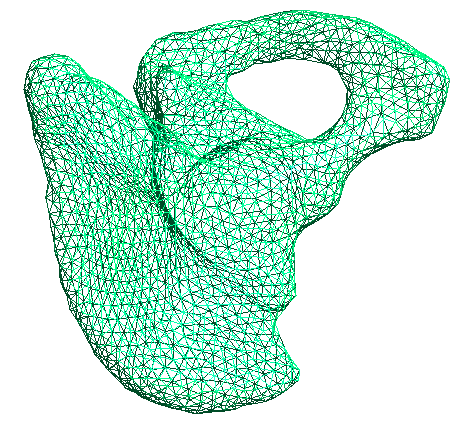
\includegraphics[width=4.5cm]{pngs/mymesh/pelvis_stl.png}
\caption{Pelvis before remesh (stl)}
\end{minipage}
\begin{minipage}[b]{.50\linewidth}
\centering
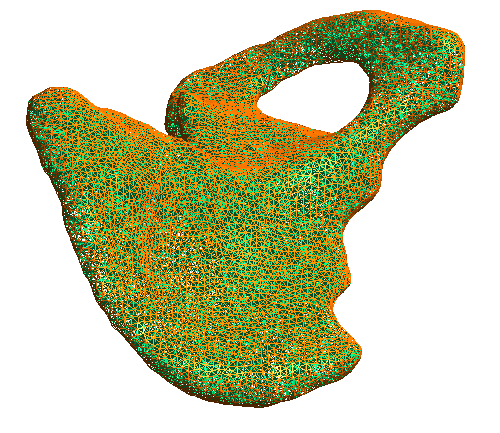
\includegraphics[width=4.5cm]{pngs/mymesh/pelvis_msh.png}
\caption{Pelvis after remesh (msh)}
\end{minipage}
\end{figure}

\end{itemize}


\section{Language for Partial Differential Equations}
\label{faq:PDE}

\subsection{What is the difference between using the "vf::project" function and solve a weak projection problem ?}

To make it clear, let's considerate that we want to project a $\mathbb{P}_1$ scalar function $\sigma$ on a $\mathbb{P}_0$ space. We have two alternatives to do it :
\begin{itemize}
\item Computing the $\mathcal{L}_2$ projection of $\sigma$ onto the space \newline
Here $kappa$ and $v$ are $\mathbb{P}_0$ functions :
\begin{lstlisting}
Matrix_M=integrate(elements(mesh), idt(kappa) * id(v));
Vector_F=integrate(elements(mesh), idv(sigma) * id(v));
\end{lstlisting}

\item Use the project function \lstinline!vf::project! \newline
This function does a nodal projection : at the dof point the projection will be \underline{exactly} equal to the projected function $\sigma$. It works as follow
\begin{lstlisting}
kappa=vf::project(P0_space, elements(mesh), idv(sigma));
\end{lstlisting}
\end{itemize}

These two projections are in general different, if you compare the values in the vector, they will be (slightly) different. However as $h \rightarrow 0$ they should both converge to the $\sigma$ function.


\subsection{How to do a quick L2 projection of an expression ?}
Let say that we have created two spaces, one scalar and one vectorial, we call them $\displaystyle{X_h}$ and $\displaystyle{X_{hVec}}$ and one wants to project some expressions on those spaces. \newline \newline
For example, we want to project $\displaystyle{(x,y) \rightarrow \sqrt{x^2 - y^2} -1}$ on the scalar space and $\displaystyle{(-2y, \cos{x})}$ on the vectorial space.
First of all, one has to create projectors for the scalar and vectorial spaces, the code reads as follow :
\begin{lstlisting}
#include <feel/feeldiscr/projector.hpp>
auto l2p = projector(Xh, Xh);
auto l2pVec = projector(XhVec, XhVec);
\end{lstlisting}
You can note that \lstinline!projector(Space, Space)! returns a \lstinline!boost::shared_ptr! on a \lstinline!Projector! object which makes projecting functions on \lstinline!Space! possible.
\newline \newline
Then, one uses the function \lstinline!Projector::project(Expression)! :
\begin{lstlisting}
auto Circle = l2p->project( sqrt( pow((vf::Px()),2.0)+ pow((vf::Py()),2.0)) - 1 );

auto F = l2pVec->project( -2 * Py() * oneX() + cos(vf::Px()) * oneY() );
\end{lstlisting}
Here you can note that the types of \lstinline!Circle! and \lstinline!F! are respectively : $X_{h}\_type::element\_type$ and $X_{hVec}\_type::element\_type$
\newline
An equivalent way to write it is to use the \lstinline!Projector::operator()(Expression)! :
\begin{lstlisting}
auto Circle = (*l2p)( sqrt( pow((vf::Px()),2.0)+ pow((vf::Py()),2.0)) - 1 );

auto F = (*l2pVec)( -2 * Py() * oneX() + cos(vf::Px()) * oneY() );
\end{lstlisting}
\lstinline!Projector::operator()! accepts many types of arguments, see \lstinline!feel/feeldiscr/projector.hpp! for details.



\subsection{How to compose \feel operators ?}

Let's considerate that we have created two spaces, one scalar $X_h$ and one vectorial $X_{hVec}$. We also have two vectors $a$ and $b$ (of type $X_{h}\_type::element\_type$).

One wants to do the following operation : $div( grad(a*b))$. The following expression is \textbf{not} yet implemented in \feel :
\begin{lstlisting}
divv( gradv( idv(a) * idv(b) ) )
\end{lstlisting}
One has to do intermediate projections to compose the operators. Using the Projector class, the code reads :
\begin{lstlisting}
#include <feel/feeldiscr/projector.hpp>

// create projectors on Xh and XhVec spaces
auto l2p = projector(Xh, Xh);
auto l2pVec = projector(XhVec, XhVec);

auto ab = l2p->project( idv(a)*idv(b) );
auto grad_ab = l2pVec->project( gradv(ab) );
auto div_grad_ab = l2p->project( divv(grad_ab) );
\end{lstlisting}
Here \lstinline!div_grad_ab! has the type $X_{h}\_type::element_type$. There is an equivalent but verboseless way to write this composition : use the \lstinline!Projector::operator()! which accepts has argument an expression or an \lstinline!element_type!. So one could write :
\begin{lstlisting}
#include <feel/feeldiscr/projector.hpp>

//create projectors on Xh and XhVec spaces
auto l2p = projector(Xh, Xh);
auto l2pVec = projector(XhVec, XhVec);

auto div_grad_ab = (*l2p)( divv( (*l2pVec)( gradv( (*l2p)(idv(a)*idv(b)) ) ) ) );
\end{lstlisting}
the * is needed before \lstinline!l2p! or \lstinline!l2pVec! since there are \lstinline!boost::shared_ptr! objects. One could also create directly \lstinline!Projector! objects :
\begin{lstlisting}
Projector<Xh_type, Xh_type> l2p(Xh, Xh);

auto ab = l2p(idv(a)*idv(b));
\end{lstlisting}


%%% Local Variables:
%%% coding: utf-8
%%% mode: latex
%%% TeX-PDF-mode: t
%%% TeX-parse-self: t
%%% x-symbol-8bits: nil
%%% TeX-auto-regexp-list: TeX-auto-full-regexp-list
%%% TeX-master: "feelpp-manual"
%%% ispell-local-dictionary: "american"
%%% End:


\chapter{Random notes}
\label{cha:random-notes}

\section{Becoming a Feel++ developer}
\label{feeldevel}
\subsection{Interest}
Becoming a \feel developer makes library improvements possible, you may have several proposals which may be usefull. Taking part of the project will enable you to commit some modifications or new applications, we will be glad to count you among us. As an open-source project under GNU licence,  you will be able to commit and participate to the entire project and its various aspects. Our aim is that each user should be involved in the library's expansion. In the following part, you will see how you can become a \feel collaborator.

\subsection{Creating RSA keys}
\label{sec:creation-rsa-keys}
At the top of the manual, you have seen how to get the sources anonymously, if you want to checkout or commit properly, you will need an account on \href{https://forge.imag.fr/}. After the administrator approval, you have to demand the rights to see the project tree. \newline \newline
Once it's done, you will have to create RSA keys to be able to connect to the server using ssh. To do that you have to type the commands : \verb|ssh-keygen| and accept the 3 questions without typing anything. The generated key is placed in \verb|~/.ssh/id_rsa.pub|, you just need to copy this file's content in your forge account. To make it, go on the Forge website and enter into your account's personnal page. At the bottom of the page, you'll have the possibility to edit your SSH keys, go into it and copy/paste the id\_rsa.pub content. Once it's done, the number of your SSH keys in that page should have increased. Now, you will be able to connect to the server within an hour.
%\verb|ssh-keygen -t dsa| and \linebreak[2] \verb|ssh-keygen -t rsa| to create the keys. After that, you have to copy the \verb|id_dsa.pub| and \verb|id_rsa.pub| files in the My Page > Account Maintenance > Edit SSH Keys section of the LJKForge website. Those files are located in the \verb|~/.ssh/| folder of your computer. You will be able to connect to the server within an hour.
\\ \\
{\bfseries Important : } If you don't have the same login on your computer as on
Forge, you must add the commands in the \verb|~/.ssh/config| file :
\begin{lstlisting}[language=sh]
host forge.imag.fr
  user <your_login_forge>
\end{lstlisting}


\subsection{Downloading the sources}
\label{sec:download-sources}

To be able to download the \feel sources, you need subversion and SSH > 1.xxx
installed on your computer. In a command prompt, go where you want \feel to be
downloaded and type the following command :
\\ \verb|svn co svn+ssh://login@scm.forge.imag.fr/var/lib/gforge/chroot/scmrepos|
\\ \verb|/svn/life/trunk/life/trunk feel|
\\ where \verb|login| is your login name in the Forge plateform.

% ---- Useless now ? the command above downloads all feel sources, included the feel-test ---------
%Then, if you want to download the feel-test sources type :
%\begin{unixcom}
% cd feel/benchmarks
%  svn co svn+ssh://login@scm.forge.imag.fr/var/lib/gforge/chroot/scmrepos/svn/feel-test/feel-test/trunk validation
%\end{unixcom}
You are now able to checkout, commit or add the file your judge usefull using \verb|svn|, please don't forget to comment on your various actions. The first commit is subject to the approbation of one of the main developers.


\section{Programming environment}
\label{sec:progr-envir}
We present here a quick list of all namespaces and librairies proposed by \feel, refer to the
tutorial which starts at chapter ~\ref{chap:getting-started} how you can use them.
\subsection{Boost C++ Libraries}
\label{sec:boost-c++-libraries}

\feel depends on a number of libraries, some are required some are optional.
Among the required libraries, The Boost C++ libraries play a very important role
as they drive or shape the  design of \feel. \feel uses in particular the
following Boost libraries:
\begin{itemize}
\item Boost.Parameter\index{Boost!Parameter} : use to provide powerful
  interfaces to \feel and third party library such as
  \begin{itemize}
  \item PETSc  for the linear, nonlinear solvers
  \item SLEPc for the eigenvalue solvers
  \item GMSH for mesh generation
  \end{itemize}
\item Boost.MPL - meta programming library : use for type computations
\item Boost.Fusion - linking meta-runtime programming: use for type computations
  used at runtime
\item Boost.Program\_Options - command-line options library : provides the
  command line options for the \feel applications as well as configuration files
\item Boost.Test - Unit testing framework ; used by the \feel testsuite
\end{itemize}

\subsection{\feel Namepaces}

\begin{itemize}
\item \lstinline!Feel!
\item \lstinline!Feel::po!
\item \lstinline!Feel::mpl!
\item \lstinline!Feel::ublas!
\item \lstinline!Feel::math!
\item \lstinline!Feel::fem!
\item \lstinline!Feel::vf!

\end{itemize}



\section{Linear Algebra with PETSC}

\subsection{Using the Petsc Backend: recommended}

Using the Petsc backend is recommended. To do that type in the command line
\begin{lstlisting}
    myprog --backend=petsc
  \end{lstlisting}
  then you can change the type of solvers and preconditioners by
  adding Petsc options at \emph{the end of the command lines}, for example
\begin{verbatim}
-pc_type lu
\end{verbatim}
  will actually solve the problem in one iteration of an iterative solver
  (p.ex. gmres).
  \begin{equation}
    \label{notes:eq:1}
    P A x = P B
  \end{equation}
  where $P \approx A^{-1}$. Here $A$ is decomposed in $LU$ form and
  (\ref{notes:eq:1}) is solved in one iteration.

\subsection{List of solvers and preconditioners}
\label{sec:list-solv-prec}

List of some iterative solvers (Krylov subspace)
\begin{itemize}
\item cg, bicg
\item gmres, fgmres, lgmres
\item bcgs, bcgsl
\item see petsc/petscksp.h for more
\end{itemize}

List of some preconditioners
\begin{itemize}
\item lu, choleski
\item jacobi, sor
\item ilu, icc
\item see petsc/petscpc.h for more
\end{itemize}

\subsection{What is going on in the solvers?}
\label{sec:what-going-solvers}

In order to monitor what is going on (iterations, residual...) Petsc
provides some monitoring options
\begin{verbatim}
-ksp_monitor
\end{verbatim}
For example
\begin{verbatim}
myprog -backend=petsc -ksp_monitor -pc_type lu
\end{verbatim}
it should show only one iteration.

See {\tiny\texttt{http://www.mcs.anl.gov/petsc/petsc-as/snapshots/petsc-current/docs/manualpages/KSP/KSPMonitorSet.html}} for more details



\section{Weak Dirichlet boudary conditions}
\label{sec:weak-dirichl-boud}

\subsection{Basic idea}

\subsubsection{Weak treatment}
  In order to treat the boundary conditions uniformly (i.e. the same
  way as Neumann and Robin Conditions), we wish to treat the Dirichlet
  BC (e.g. $u=g$) weakly.

  \begin{remark}{Initial Idea}
    add the penalisation term $\int_{\partial \Om{}} \mu( u - g
    )$ where $\mu$ is a constant. But this is not enough, this is not consistent with the
    initial formulation.
  \end{remark}

  One can use the Nitsche ``trick'' to implement weak Dirichlet conditions.
  \begin{itemize}
  \item write the equations in conservative form (i.e. identify the flux);
  \item add the terms to ensure consistency (i.e the flux on the boundary);
  \item symmetrize to ensure adjoint consistency;
  \item add a penalisation term with factor $\gamma (u-g)/h$ that ensures
    that the solution will be set to the proper value at the boundary;
  \end{itemize}


\subsubsection{Penalisation parameter}
    \begin{remark}{Choosing $\gamma$}
    $\gamma$ must be chosen such that the coercivity(or inf-sup)
    property is satisfied. Difficult to do in general. Increase
    $\gamma$ until the BC are properly satisfied, e.g. start with
    $\gamma=1$, typical values are between 1 and 10.

    The choice of $\gamma$ is a problem specially when $h$ is small.
  \end{remark}



\subsubsection{Advantages, disadvantages}
      \begin{remark}{Weak treatment: Advantages}
        \begin{itemize}
        \item uniform(weak) treatment of all boundary conditions type
        \item if boundary condition is independant of time, the terms
          are assembled once for all
        \item the boundary condition is not enforced exactely but the
          convergence order remain optimal
        \end{itemize}
      \end{remark}
      \begin{remark}{Weak treatment: Disadvantages}
        \begin{itemize}
        \item Introduction of the penalisation parameter $\gamma$ that
          needs to be tweaked
        \end{itemize}
      \end{remark}

\subsubsection{Advantages, disadvantages}
  \begin{remark}{Strong treatment: Advantages}
    \begin{itemize}
    \item Enforce exactely the boundary conditions
    \end{itemize}
  \end{remark}
  \begin{remark}{Strong treatment : Disadvantages}
    \begin{itemize}
    \item Need to modify the matrix once assembled to reflect that
      the Dirichlet degree of freedom are actually known. Then
          even if the boundary condition is independant of time, at
          every time step if there are terms depending on time that
          need reassembly (e.g. convection) the strong treatment needs to be reapplied.
        \item it can be expensive to apply depending on the type of
          sparse matrix used, for example using CSR format setting
          rows to 0 except on the diagonal to 1 is not expensive but
          one must do that also for the columns associated with each
          Dirichlet degree of freedom and that is expensive.
        \end{itemize}
      \end{remark}

\subsection{Laplacian}
\subsubsection{Example: Laplacian}
  \begin{equation}
    \label{notes:eq:44}
    -\Delta u = f (\text{non conservative}),\ -\nabla\cdot( \nabla u )= f (\text{conservative}),\ u=g|_{\partial \Omega}
  \end{equation}
  the flux is vector $\nabla u$

  \begin{equation}
    \label{notes:eq:51}
    \int_\Omega \nabla u \cdot \nabla v + \int_{\partial \Om{}} \underbrace{-\frac{\partial u}{\partial n}v}_{\text{integration by part}} \underbrace{-\frac{\partial v}{\partial n} u}_{\text{adjoint consistency: symetrisation}}  + \underbrace{\frac{\gamma}{h} u v}_{\text{penalisation: enforce Dirichlet condition}}
  \end{equation}
  \begin{equation}
    \label{notes:eq:52}
    \int_\Omega f \nabla v + \int_{\partial \Om{}} (\underbrace{-\frac{\partial v}{\partial n} g}_{\text{adjoint consistency}} + \underbrace{\frac{\gamma}{h} v) g}_{\text{penalisation: enforce Dirichlet condition}}
  \end{equation}


\subsubsection[containsverbatim]{Example: Laplacian}
  \begin{lstlisting}
// bilinear form (left hand side)
form2( Xh, Xh, D ) +=
integrate( boundaryfaces(mesh), im_type(),
           -(gradt(u)*N())*id(v) // integration by part
           -(grad(v)*N())*idt(u) // adjoint consistency
           +gamma*id(v)*idt(u)/hFace()); // penalisation
// linear form (right hand side)
form1( Xh, F ) +=
integrate( boundaryfaces(mesh), im_type(),
           -(grad(v)*N())*g // adjoint consistency
           +gamma*id(v)*g/hFace()); // penalisation
  \end{lstlisting}


\subsection{Convection-Diffusion}
\subsubsection{Example: Convection-Diffusion}
  \begin{remark}{Convection Diffusion}
    Consider now the following problem, find $u$ such that
    \begin{equation}
      \label{notes:eq:45}
      -\Delta u + \mathbf{c} \cdot \nabla u  = f,\quad u = g|_{\partial \Om{}},\quad \nabla \cdot \mathbf{c} = 0
    \end{equation}
    under conservative form the equation reads
    \begin{equation}
      \label{notes:eq:2}
      \nabla \cdot ( -\nabla u + \mathbf{c} u ) = f,\quad u = g|_{\partial \Om{}},\quad \nabla \cdot \mathbf{c} = 0
    \end{equation}
    the flux vector field is $\mathbf{F}=-\nabla u + \mathbf{c} u$. Note that
    here the condition, $\nabla \cdot \mathbf{c} = 0$ was crucial to
    expand $\nabla \cdot (\mathbf{c} u )$ into $\mathbf{c} \cdot \nabla u$ since
    \begin{equation}
      \label{notes:eq:3}
      \nabla \cdot (\mathbf{c} u ) = \mathbf{c} \cdot \nabla u + \underbrace{u \nabla \cdot \mathbf{c}}_{=0}
    \end{equation}
  \end{remark}


\subsubsection{Weak formulation for convection diffusion}
  Multiplying by any test function $v$ and integration by
  part of (\ref{notes:eq:2}) gives
  \begin{equation}
    \label{notes:eq:4}
    \int_\Omega \nabla u \cdot \nabla v + (\mathbf{c} \cdot \nabla u)v + \int_{\partial \Omega} (\mathbf{F}\cdot \mathbf{n}) v = \int_\Omega f v
  \end{equation}
  where $\mathbf{n}$ is the outward unit normal to $\partial
  \Omega$. We now introduce the penalisation term that will ensure
  that $u \rightarrow g$ as $h \rightarrow 0$ on $\partial \Omega$. (\ref{notes:eq:4}) reads now
  \begin{equation}
    \label{notes:eq:5}
    \int_\Omega \nabla u \cdot \nabla v + (\mathbf{c} \cdot \nabla u)v + \int_{\partial \Omega} (\mathbf{F}\cdot \mathbf{n}) v + \mathbf{\frac{\gamma}{h} u v}  = \int_\Omega f v + \mathbf{\int_{\partial \Omega} \frac{\gamma}{h} g v}
  \end{equation}

  Finally we incorporate the symetrisation of the bilinear form to ensure adjoint consistency and hence proper convergence order
  \begin{equation}
    \label{notes:eq:6}
    \begin{split}
      \int_\Omega \nabla u \cdot \nabla v + (\mathbf{c} \cdot \nabla u)v +
      \int_{\partial \Omega} ((-\nabla u + \mathbf{c} u)\cdot \mathbf{n}) v+ \mathbf{((-\nabla v + \mathbf{c} v)\cdot \mathbf{n}) u} + \frac{\gamma}{h} u v  = \\
      \int_\Omega f v + \int_{\partial \Omega} \mathbf{((-\nabla v + \mathbf{c} v)\cdot \mathbf{n}) g}+ \frac{\gamma}{h} g v
    \end{split}
  \end{equation}


\subsubsection[containsverbatim]{Example: Convection-Diffusion}
  \begin{lstlisting}
// bilinear form (left hand side)
form2( Xh, Xh, D ) +=
integrate( boundaryfaces(mesh), im_type(),
           // integration by part
           -(gradt(u)*N())*id(v) + (idt(u)*trans(idv(c))*N())*id(v)
           // adjoint consistency
           -(grad(v)*N())*idt(u) + (id(v)*trans(idv(c))*N())*idt(u)
           // penalisation
           +gamma*id(v)*idt(u)/hFace());
// linear form (right hand side)
form1( Xh, F ) +=
integrate( boundaryfaces(mesh), im_type(),
           // adjoint consistency
           -(grad(v)*N())*g + (id(v)*trans(idv(c))*N())*g
           // penalisation
           +gamma*id(v)*g/hFace());
  \end{lstlisting}


\subsection{Stokes}
\subsubsection{Example: Stokes}
  \begin{remark}{Stokes}
    Consider now the following problem, find $(\mathbf{u},p)$ such that
    \begin{equation}
      \label{notes:eq:45}
      -\Delta \mathbf{u} + \nabla p  = \mathbf{f},\quad \mathbf{u} = \mathbf{g}|_{\partial \Om{}},\quad \nabla \cdot \mathbf{u} = 0
    \end{equation}
    under conservative form the equation reads
    \begin{eqnarray}
      \nabla \cdot ( -\nabla \mathbf{u} + p \mathbb{I} ) &= \mathbf{f},\label{notes:eq:8}\\
      \nabla \cdot \mathbf{u} &= 0,\label{notes:eq:10}\\
      \mathbf{u} &= \mathbf{g}|_{\partial \Om{}}\label{notes:eq:11}
    \end{eqnarray}
    where $\mathbb{I}(\mathbf{x})=
    \begin{pmatrix}
      1 & 0\\
      0 & 1
    \end{pmatrix}\text{(in 2D)}
    \ \forall \mathbf{x} \in \Omega$ is the identity tensor(matrix) field $\in
    \mathbb{R}^{d\times d}$. The flux tensor field is
    $\mathbf{F}=-\nabla \mathbf{u} + p\mathbb{I}$. Indeed we have  the
    following relation, if $\mathbb{M}$ is a tensor (rank 2) field and $\mathbf{v}$ is a vector field
    \begin{equation}
      \label{notes:eq:12}
      \nabla \cdot ( \mathbb{M} \mathbf{v} ) = (\nabla \cdot \mathbb{M}) \cdot \mathbf{v} + \mathbb{M} \colon (\nabla \mathbf{v})
    \end{equation}
    where $\mathbb{M} \colon (\nabla \mathbf{v}) =
    \mathrm{trace}(\mathbb{M}*\nabla \mathbf{v}^T)$, $*$ is the
    matrix-matrix multiplication and $\nabla \cdot \mathbb{M}$ is the
    vector field with components the divergence of each row of
    $\mathbb{M}$. For example $\nabla \cdot (p\ \mathbb{I})=\nabla \cdot
    \begin{pmatrix}
      p & 0 \\
      0 & p
    \end{pmatrix}(\text{in 2D}) =  \nabla p$.
  \end{remark}


\subsubsection{Weak formulation for Stokes}
  Taking the scalar product of (\ref{notes:eq:8}) by any test function
  $\mathbf{v}$ (associated to velocity) and multiplying (\ref{notes:eq:10})
  by any test function $q$ (associated to pressure), the variational
  formulation of (\ref{notes:eq:8}) reads, thanks to~(\ref{notes:eq:12}),
  \begin{equation}
    \label{notes:eq:9}
    \int_\Omega \nabla \mathbf{u} \colon \nabla \mathbf{v} +  p \nabla \cdot \mathbf{v} + \int_{\partial \Omega} ( (-\nabla \mathbf{u} + p\mathbb{I}) \mathbf{n}) \cdot \mathbf{v} = \int_\Omega \mathbf{f} \cdot \mathbf{v}
  \end{equation}
  where $\mathbf{n}$ is the outward unit normal to $\partial
  \Omega$. We now introduce the penalisation term that will ensure
  that $\mathbf{u} \rightarrow \mathbf{g}$ as $h \rightarrow 0$ on $\partial \Omega$. (\ref{notes:eq:9}) reads now
  \begin{equation}
    \label{notes:eq:14}
    \int_\Omega \nabla \mathbf{u} \colon \nabla \mathbf{v} +  p \nabla \cdot \mathbf{v} + \int_{\partial \Omega} ((-\nabla \mathbf{u} + p\mathbb{I}) \mathbf{n})\cdot \mathbf{v} + \mathbf{\frac{\gamma}{h} \mathbf{u}\cdot \mathbf{v}}  = \int_\Omega \mathbf{f} \cdot \mathbf{v} + \mathbf{\int_{\partial \Omega} \frac{\gamma}{h} \mathbf{g} \cdot \mathbf{v}}
  \end{equation}

  Finally we incorporate the symetrisation of the bilinear form to ensure adjoint consistency and hence proper convergence order
  \begin{equation}
    \label{notes:eq:15}
    \begin{split}
      \int_\Omega \nabla \mathbf{u} \colon \nabla \mathbf{v} +  p \nabla \cdot \mathbf{v} +
      \int_{\partial \Omega} ((-\nabla \mathbf{u} + p\mathbb{I}) \mathbf{n})\cdot \mathbf{v} + ((-\nabla \mathbf{v} + q\mathbb{I}) \mathbf{n})\cdot \mathbf{u} + \frac{\gamma}{h} \mathbf{u}\cdot \mathbf{v} = \\
      \int_\Omega \mathbf{f} \cdot \mathbf{v} + \int_{\partial \Omega} ((-\nabla \mathbf{v} + q\mathbb{I}) \mathbf{n})\cdot \mathbf{g} + \frac{\gamma}{h} \mathbf{g} \cdot \mathbf{v}
    \end{split}
  \end{equation}


\subsubsection[containsverbatim]{Example: Stokes}
  \begin{lstlisting}
    // total stress tensor (trial)
    AUTO( SigmaNt, (-idt(p)*N()+mu*gradt(u)*N()) );
    // total stress tensor (test)
    AUTO( SigmaN, (-id(p)*N()+mu*grad(v)*N()) );
    // linear form (right hand side)
    form1( Xh, F ) +=
    integrate( boundaryfaces(mesh), im,
               trans(g)*(-SigmaN+gamma*id(v)/hFace() ) );
    // bilinear form (left hand side)
    form2( Xh, Xh, D )+=
    integrate( boundaryfaces(mesh), im,
               -trans(SigmaNt)*id(v)
               -trans(SigmaN)*idt(u)
               +gamma*trans(idt(u))*id(v)/hFace() );
  \end{lstlisting}



\section{Stabilisation techniques}

\subsection{Convection dominated flows}

Consider this type of problem
\begin{equation}
  \label{notes:eq:46}
  -\epsilon \Delta u + \mathbf{c} \cdot \nabla u + \gamma u = f,\quad \nabla \cdot \mathbf{c} = 0
\end{equation}
Introduce $\mathrm{Pe}=\frac{|\mathbf{c}|h}{\epsilon}$ the \emph{Péclet}
number. The dominating convection occurs when, on at least some cells,
$\mathrm{Pe} >> 1$. We talk about singularly (i.e. $\epsilon << h$)
perturbed flows.

Without doing anything wiggles occur. There are remedies  so
called \emph{Stabilisation Methods}, here some some examples:
\begin{itemize}
\item Artificial diffusion (streamline diffusion) (SDFEM)
\item Galerkin Least Squares method (GaLS)
\item Streamline Upwind Petrov Galerkin (SUPG)
\item Continuous Interior Penalty methods (CIP)
\end{itemize}

\subsection{The CIP methods}
  Add the term
  \begin{equation}
    \label{notes:eq:47}
    \sum_{F \in \Gamma_\mathrm{int} } \int_{F} \gamma\ h_F^2\ |\mathbf{c} \cdot \mathbf{n}|\  [\nabla u]  [\nabla v]
  \end{equation}
  where $\Gamma_\mathrm{int}$ is the set of internal faces where the
  $\mathrm{Pe}>>1$ (typically it is applied to all internal faces) and
  \begin{equation}
    \label{notes:eq:50}
    [\nabla u] = \nabla u \cdot \mathbf{n}|_1 + \nabla u \cdot \mathbf{n}|_2
  \end{equation}
  is the jump of $\nabla u$(scalar valued) across the face.  In the
  case of scalar valued functions
  \begin{equation}
    \label{notes:eq:53}
    [u] = u \mathbf{n}|_1 + u \mathbf{n}|_2
  \end{equation}
  \begin{remark}[Choice for $\gamma$]
    $\gamma$ can be taken in the range $[1e-2;1e-1]$. A typical value is $2.5e-2$.
  \end{remark}


\begin{lstlisting}
    // define the stabilisation coefficient expression
    AUTO( stab_coeff , ($\gamma_\beta$ abs(trans(N())*idv(beta)))*
                        vf::pow(hFace(),2.0));

    // assemble the stabilisation operator
    form2( Xh, Xh, M ) +=
     integrate(
        // internal faces of the mesh
        internalfaces(Xh->mesh()),
        // integration method
        _Q<OrderOfPolynomialToBeIntegratedExactely>,
        // stabilisation term
        stab_coeff*(trans(jumpt(gradt(u)))*jump(grad(v))));
\end{lstlisting}

\section{Interpolation}

In order to interpolate a function defined on one domain to another domain, one
can use the \lstinline{interpolate} function. The basis function of the image
space must be of \lstinline{Lagrange} type.

\begin{lstlisting}
typedef bases<Lagrange<Order, Vectorial> > basis_type; // velocity
typedef FunctionSpace<mesh_type, basis_type, value_type> space_type;
// ...
space_ptrtype Xh = space_type::New( mesh1 );
element_type u( Xh, "u" );
space_ptrtype Yh = space_type::New( mesh2 );
element_type v( Yh, "v" );

// interpolate u on mesh2 and store the result in v
interpolate( Yh, u, v );
\end{lstlisting}

%%% Local Variables:
%%% coding: utf-8
%%% mode: latex
%%% TeX-PDF-mode: t
%%% TeX-parse-self: t
%%% x-symbol-8bits: nil
%%% TeX-auto-regexp-list: TeX-auto-full-regexp-list
%%% TeX-master: "feelpp-manual"
%%% ispell-local-dictionary: "american"
%%% End:


\include{gfdl}



%%\chapter*{List of Authors and Contributors}

\begin{itemize}
\item
  Christophe Prud'homme (Université Joseph Fourier)
\end{itemize}


\section{Master students}

\begin{itemize}
\item Baptiste Morin (UJF-Polytech)
\end{itemize}

%%% Local Variables:
%%% coding: utf-8
%%% mode: latex
%%% TeX-PDF-mode: t
%%% TeX-parse-self: t
%%% x-symbol-8bits: nil
%%% TeX-auto-regexp-list: TeX-auto-full-regexp-list
%%% TeX-master: "feelpp-manual"
%%% ispell-local-dictionary: "american"
%%% End:


\backmatter

\printindex

\nocite{*}
\bibliographystyle{plain}
\bibliography{../biblio/feelpp-manual,../biblio/feelpp,../biblio/feelpp-thesis}




\end{document}
%%% Local Variables:
%%% coding: utf-8
%%% mode: latex
%%% TeX-PDF-mode: t
%%% TeX-parse-self: t
%%% x-symbol-8bits: nil
%%% TeX-auto-regexp-list: TeX-auto-full-regexp-list
%%% TeX-master: t
%%% ispell-local-dictionary: "american"
%%% End:

